\section{Resultados}

  \subsubsection*{Experimento 1: Posición de la isoterma según granularidad}

    Para ambos casos se consideraron instancias de prueba con los siguientes parámetros: $r_i = 30$, $r_e = 60$, $T_i = 1500$, $iso = 500$. Se utilizó una temperatura externa constante en todos los puntos $(r_e, \theta)$ de la discretización, ($T_e(\theta) = 50$).

    En primer lugar, se calculó la solución del sistema y la posición estimada de la isoterma para una discretización considerablemente granular, con $m + 1 = 70$ y $n = 90$, para utilizar como caso de contraste. Reproducimos los gráficos que representan las temperaturas calculadas para todos los puntos de la discretización y la ubicación estimada de la isoterma.

    {\centering \begin{tabular}{cc}
      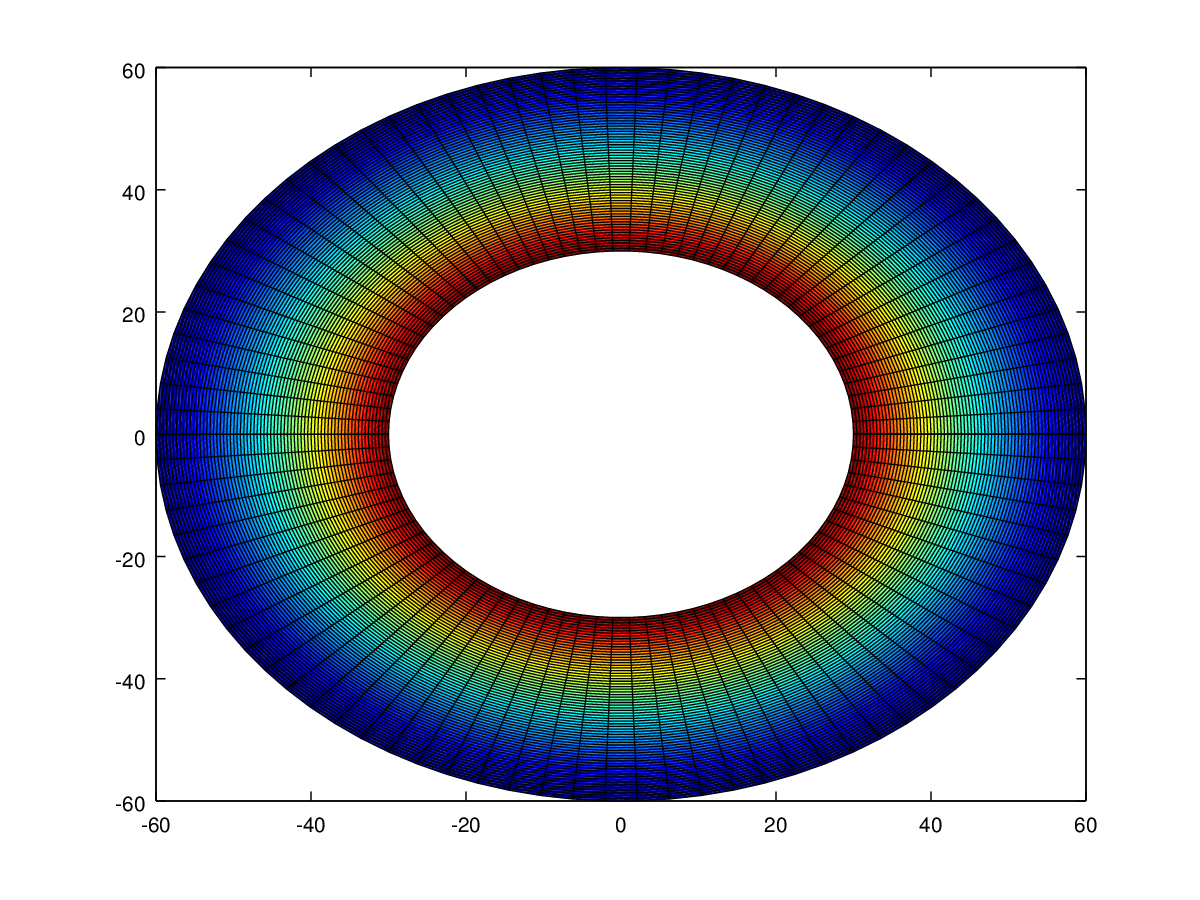
\includegraphics[height=5cm]{graficos/1/1-real.png} & 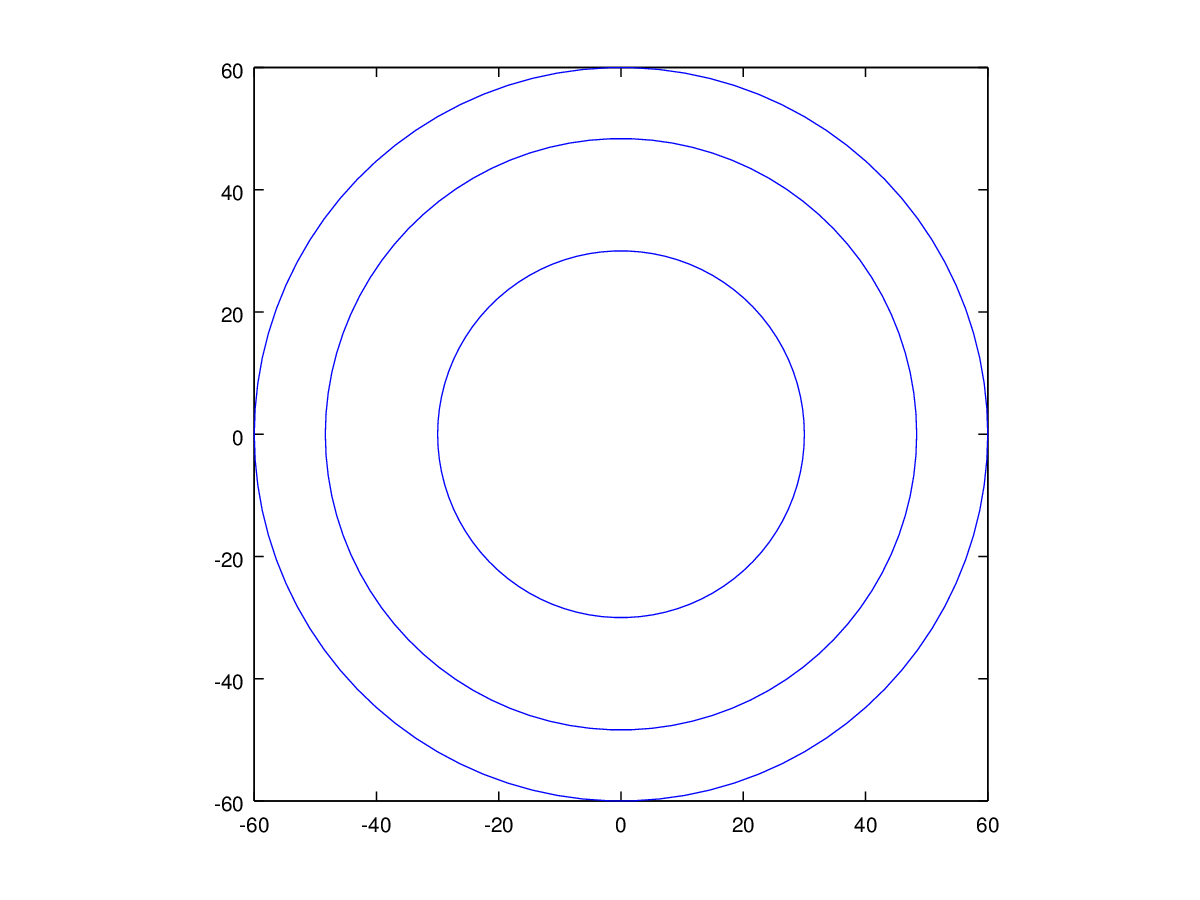
\includegraphics[height=5cm]{graficos/1/1-real-iso.png} \\
      {\small Temperaturas obtenidas} &
      {\small Posición estimada de la isoterma 500{\degree}C} \\
    \end{tabular}}

    \paragraph{Caso A} Se mantuvo constante la cantidad de radios de la discretización $m + 1 = 70$, y se tomaron instancias con diferentes cantidades de ángulos, para $n = 3, 5, 8, 10, 30, 50, 70$. Los gráficos que incluimos representan los resultados obtenidos para $n = 5, 10, 50$, reflejando las temperaturas calculadas y la ubicación estimada de la isoterma (en azul), comparada con la obtenida para el caso de contraste (en verde).

    {\centering \begin{tabular}{ccc}
      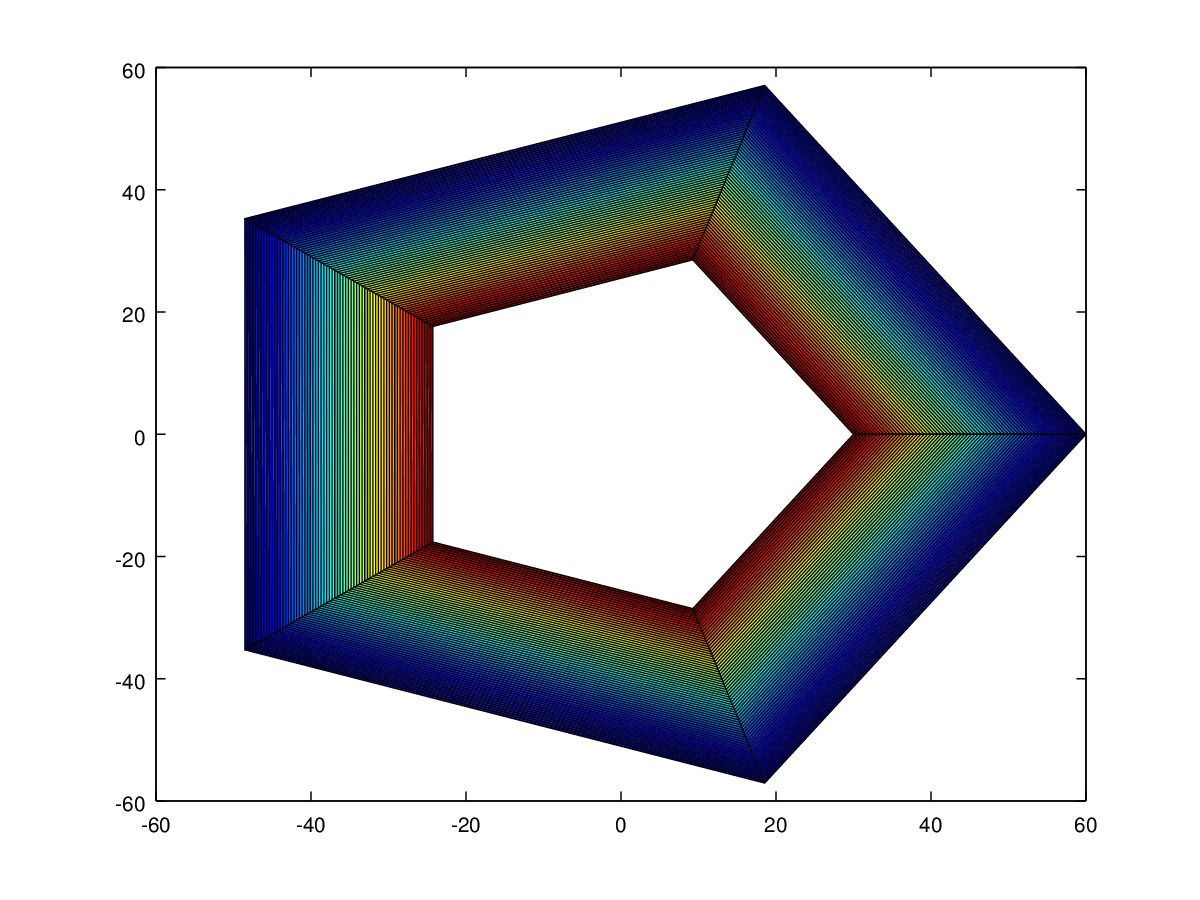
\includegraphics[width=4.5cm]{graficos/1/1a-5.png} &
      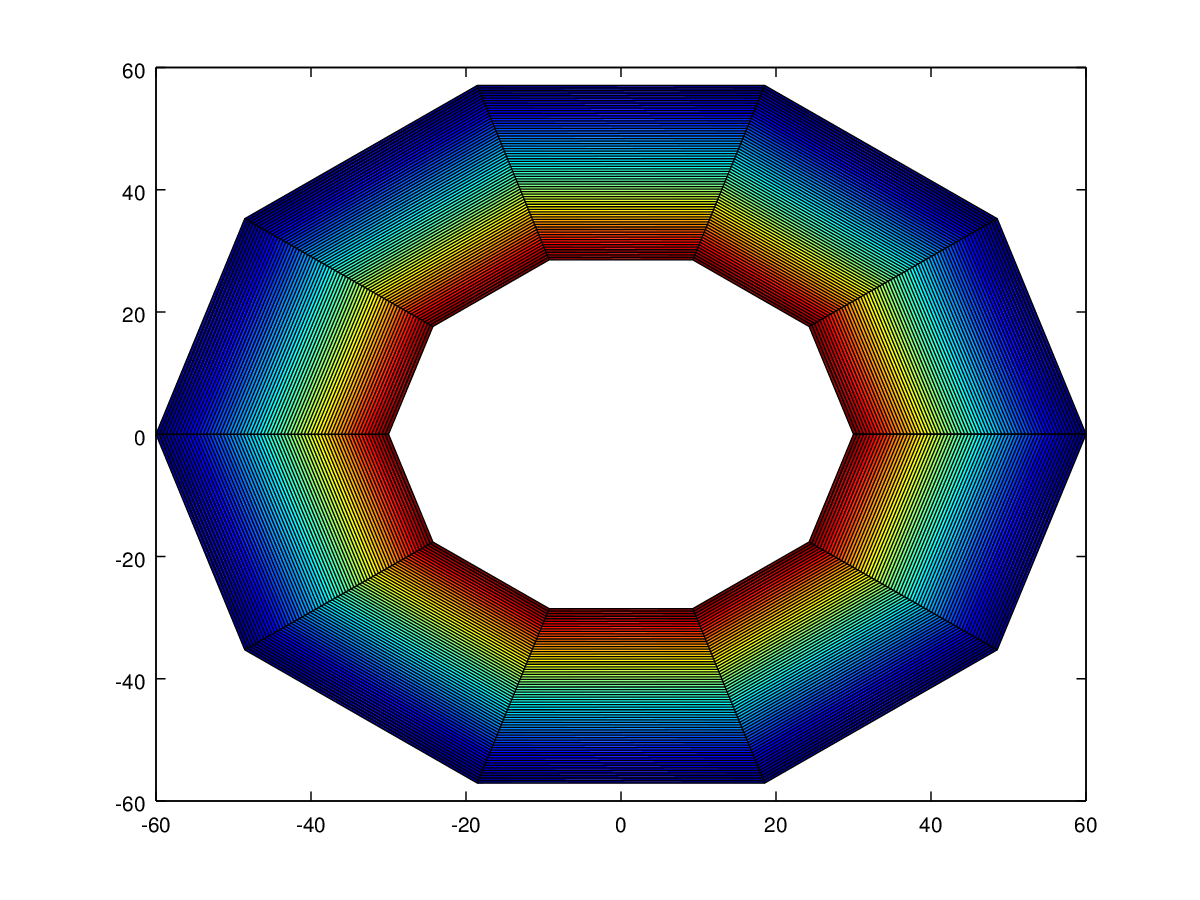
\includegraphics[width=4.5cm]{graficos/1/1a-10.png} &
      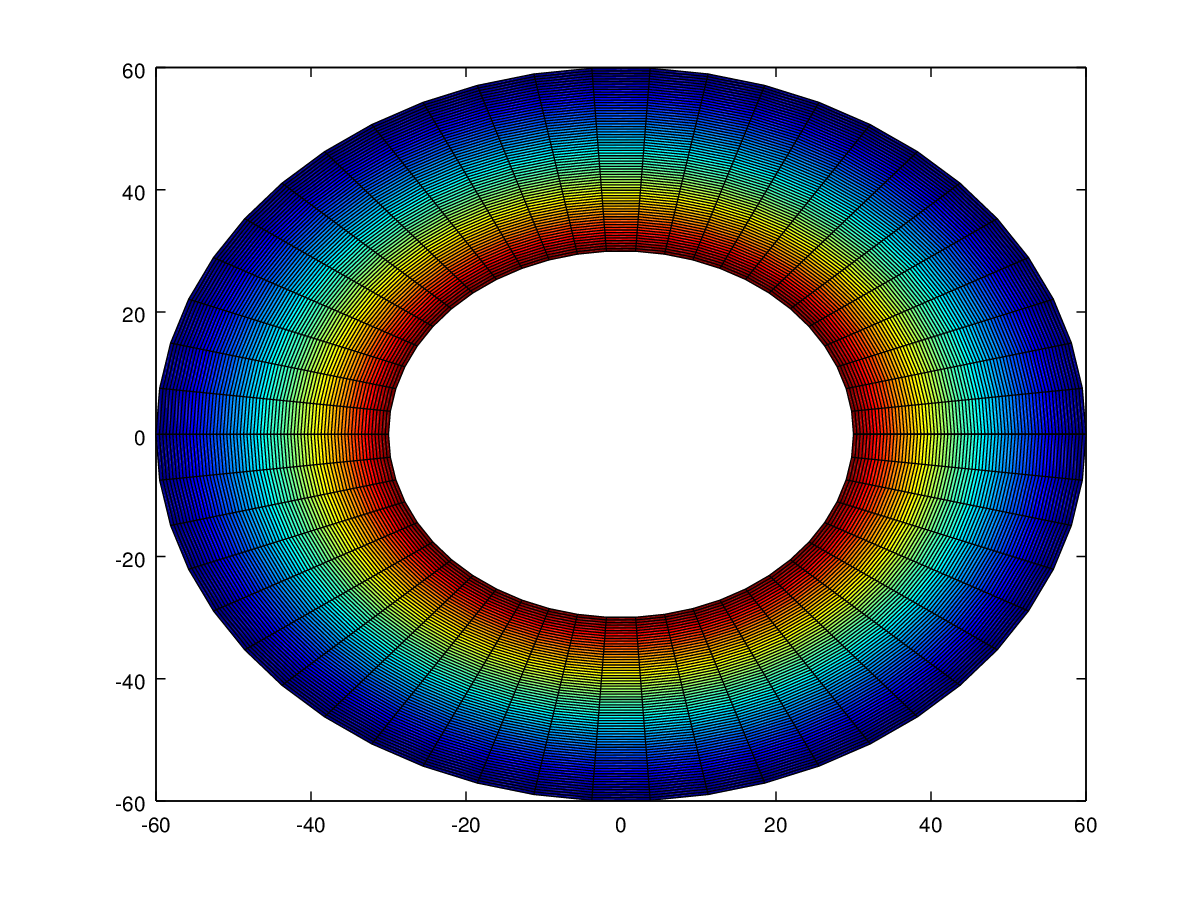
\includegraphics[width=4.5cm]{graficos/1/1a-50.png} \\
      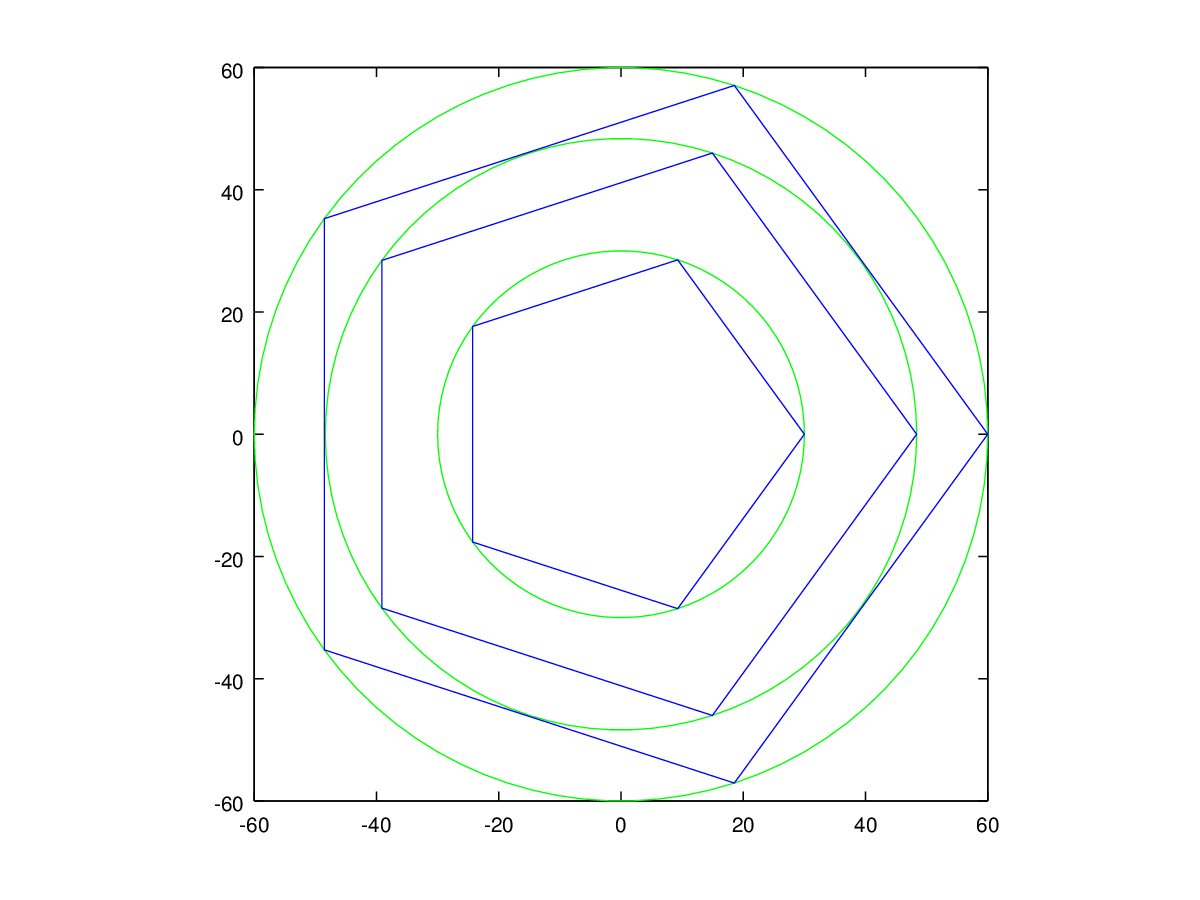
\includegraphics[width=4.5cm]{graficos/1/1a-5-iso.png} &
      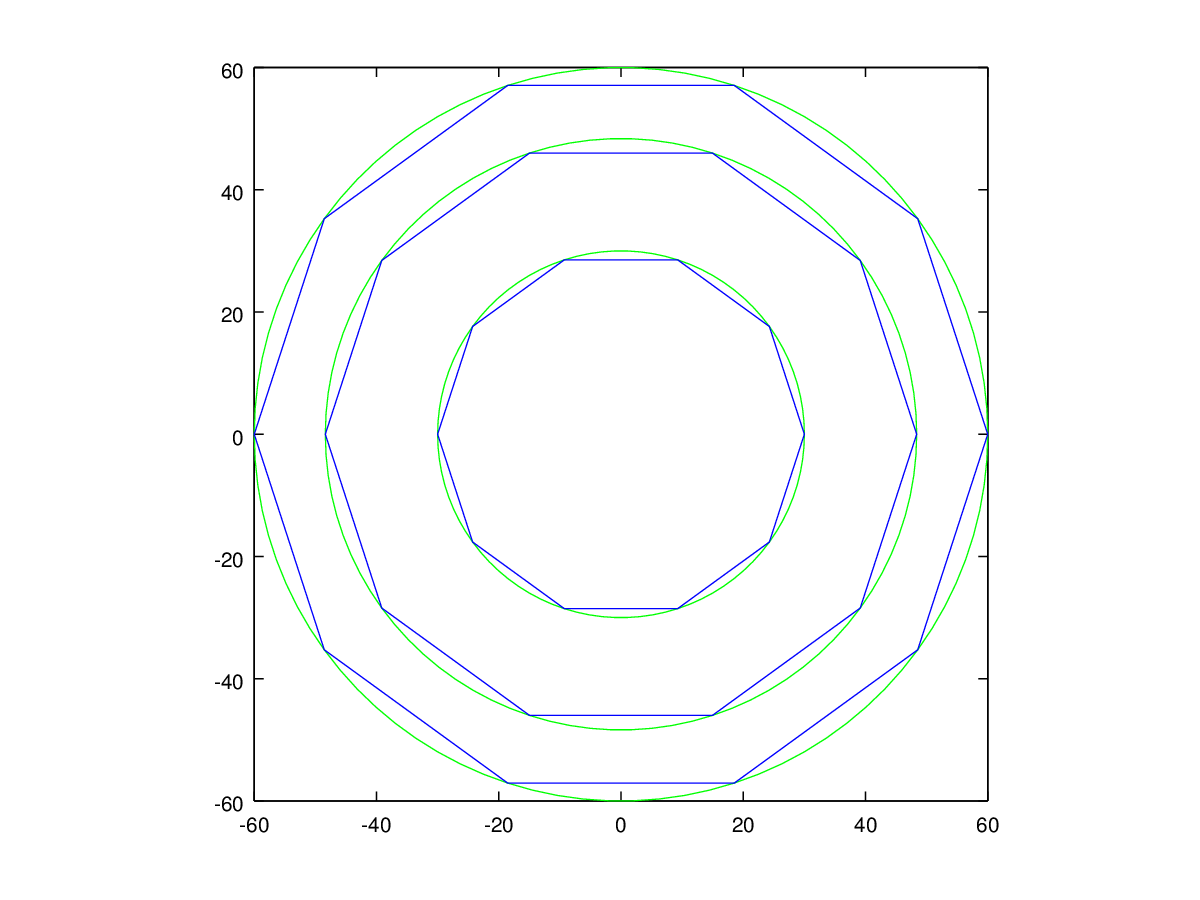
\includegraphics[width=4.5cm]{graficos/1/1a-10-iso.png} &
      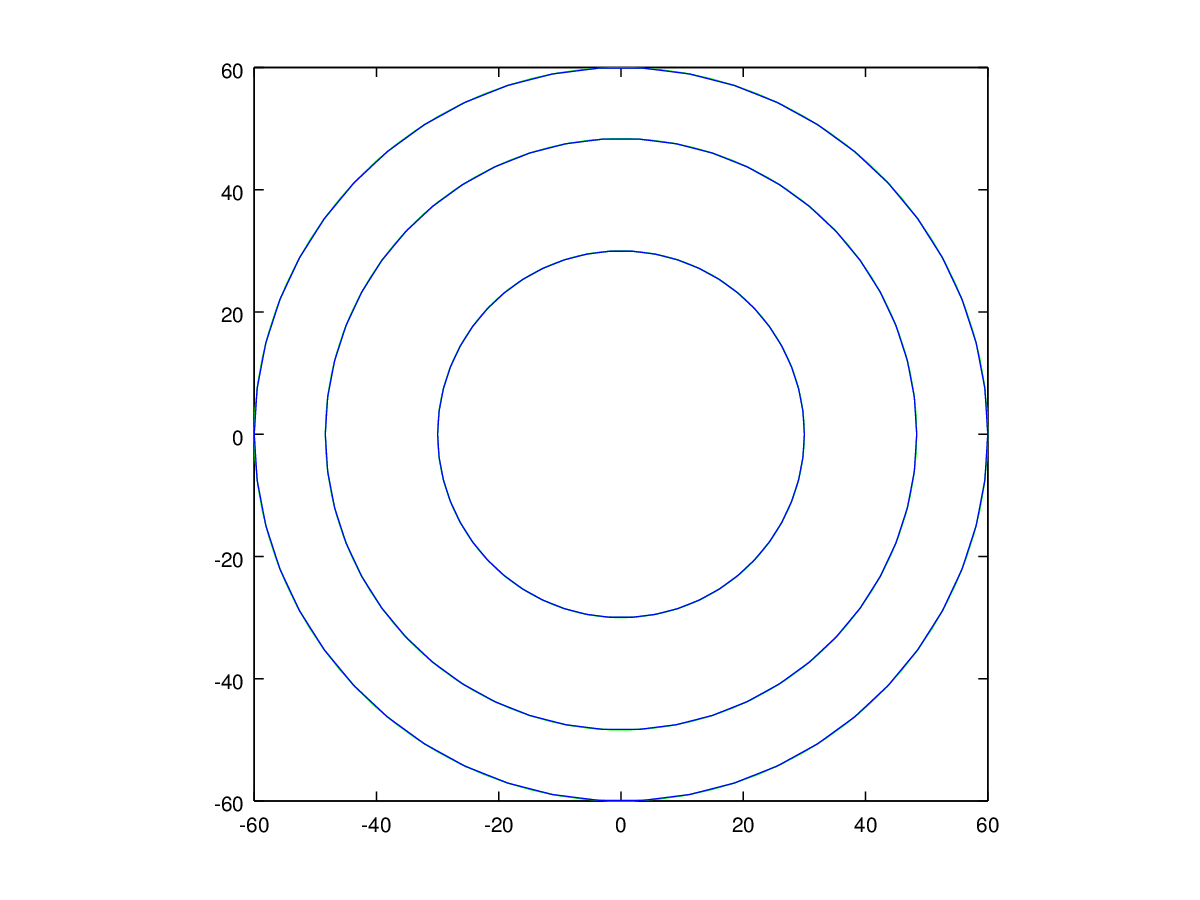
\includegraphics[width=4.5cm]{graficos/1/1a-50-iso.png} \\
      {\small $n = 5$} &
      {\small $n = 10$} &
      {\small $n = 50$} \\
    \end{tabular}}

    \paragraph{Caso B} Se mantuvo constante la cantidad de ángulos de la discretización $n = 90$, y se tomaron instancias con diferentes cantidades de ángulos, para $m + 1 = 3, 5, 8, 10, 30, 50$. Los gráficos que incluimos representan los resultados obtenidos para $m + 1 = 3, 8, 30$, reflejando las temperaturas calculadas y la ubicación estimada de la isoterma (en azul), comparada con la obtenida para el caso de contraste (en verde).

    {\centering \begin{tabular}{ccc}
      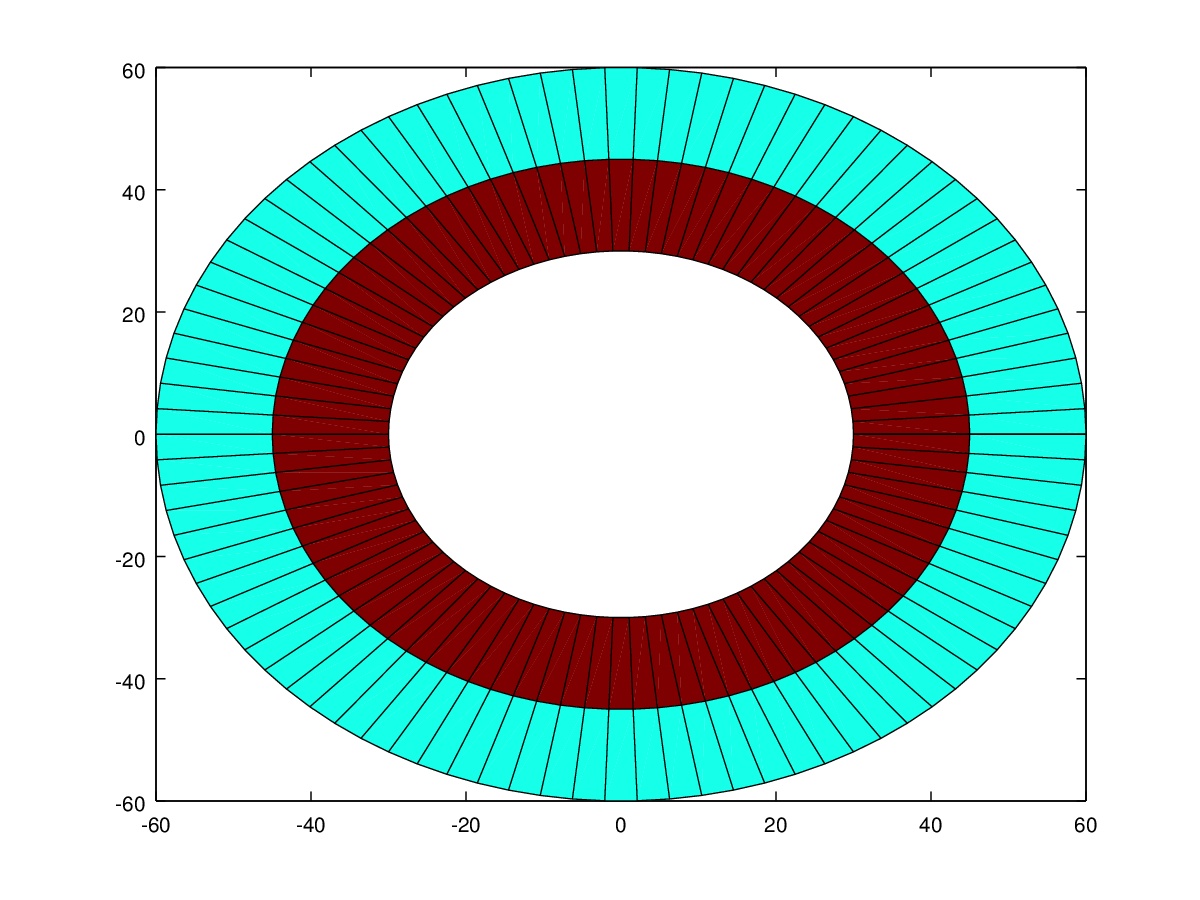
\includegraphics[width=4.5cm]{graficos/1/1b-3.png} &
      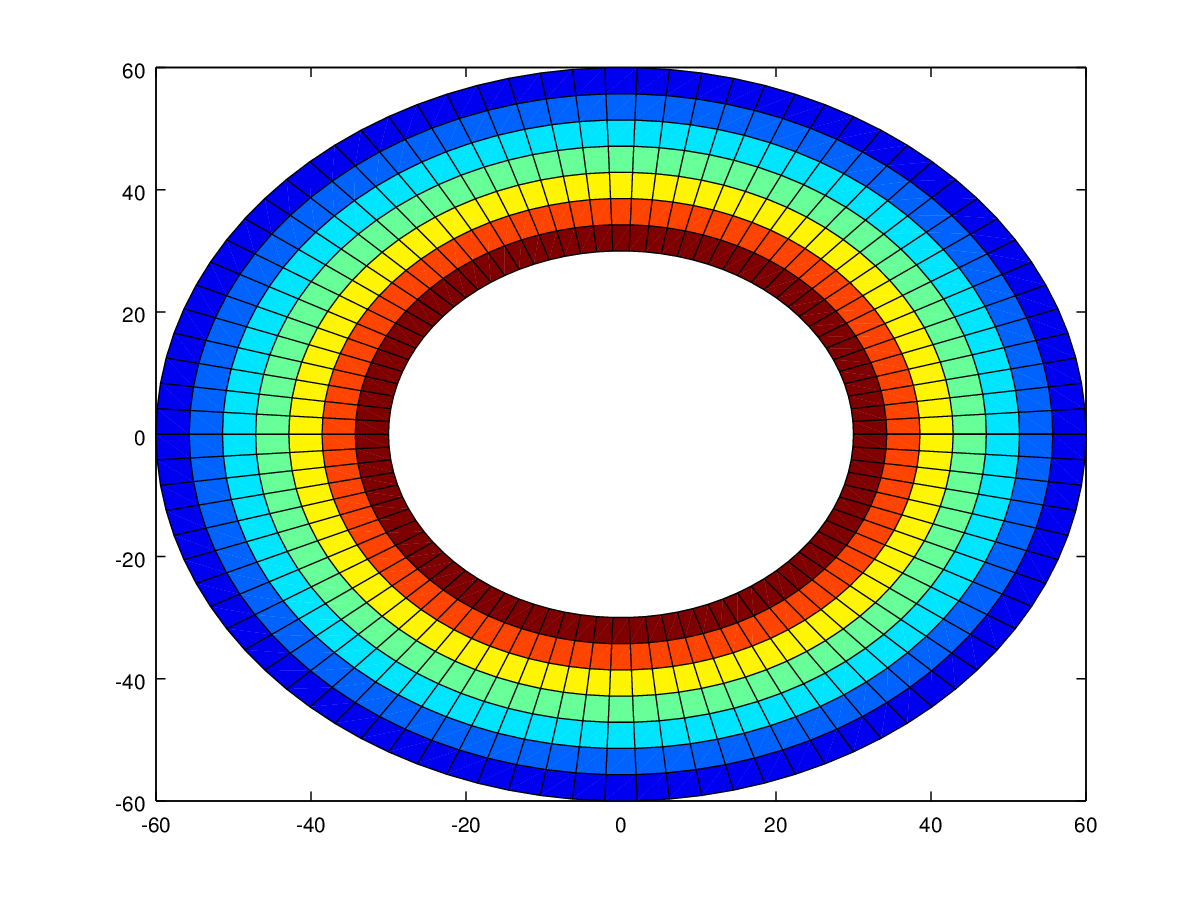
\includegraphics[width=4.5cm]{graficos/1/1b-8.png} &
      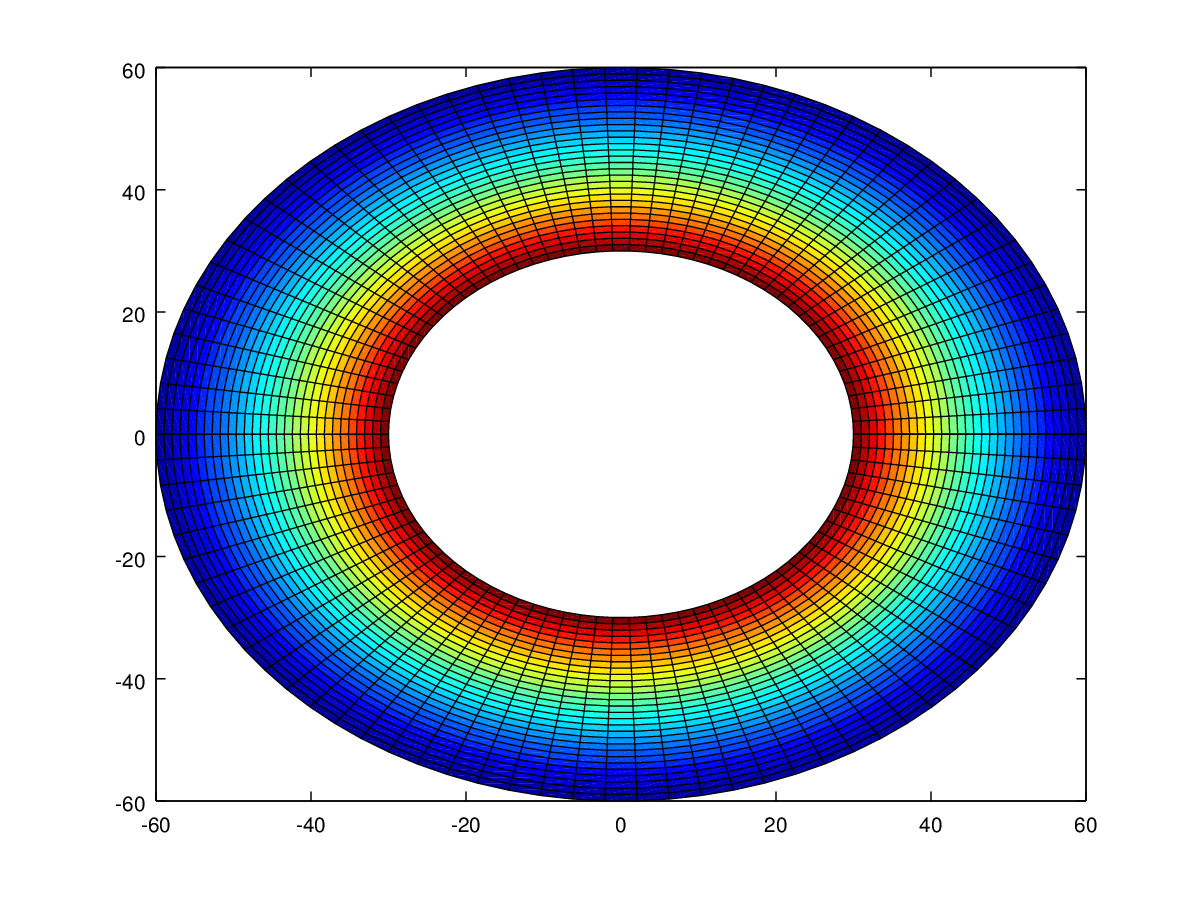
\includegraphics[width=4.5cm]{graficos/1/1b-30.png} \\
      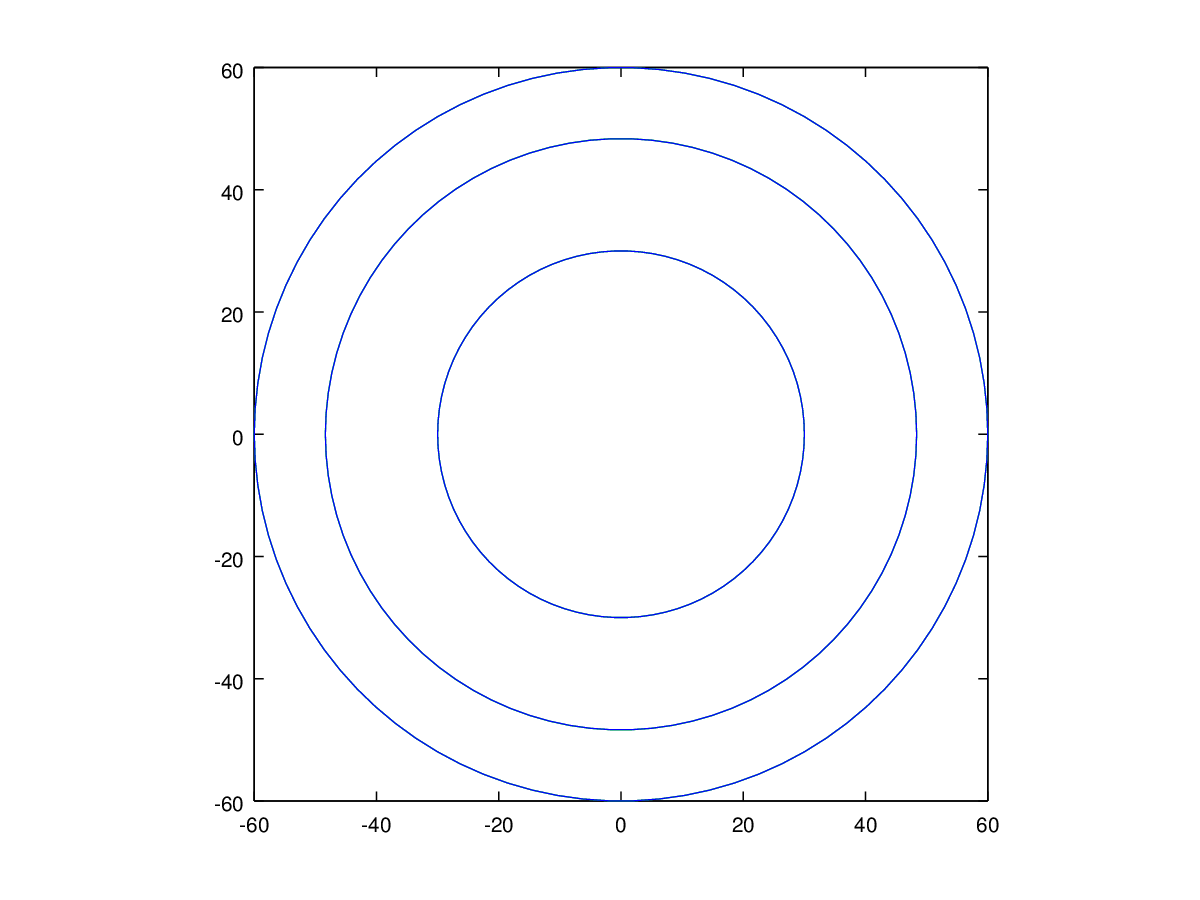
\includegraphics[width=4.5cm]{graficos/1/1b-3-iso.png} &
      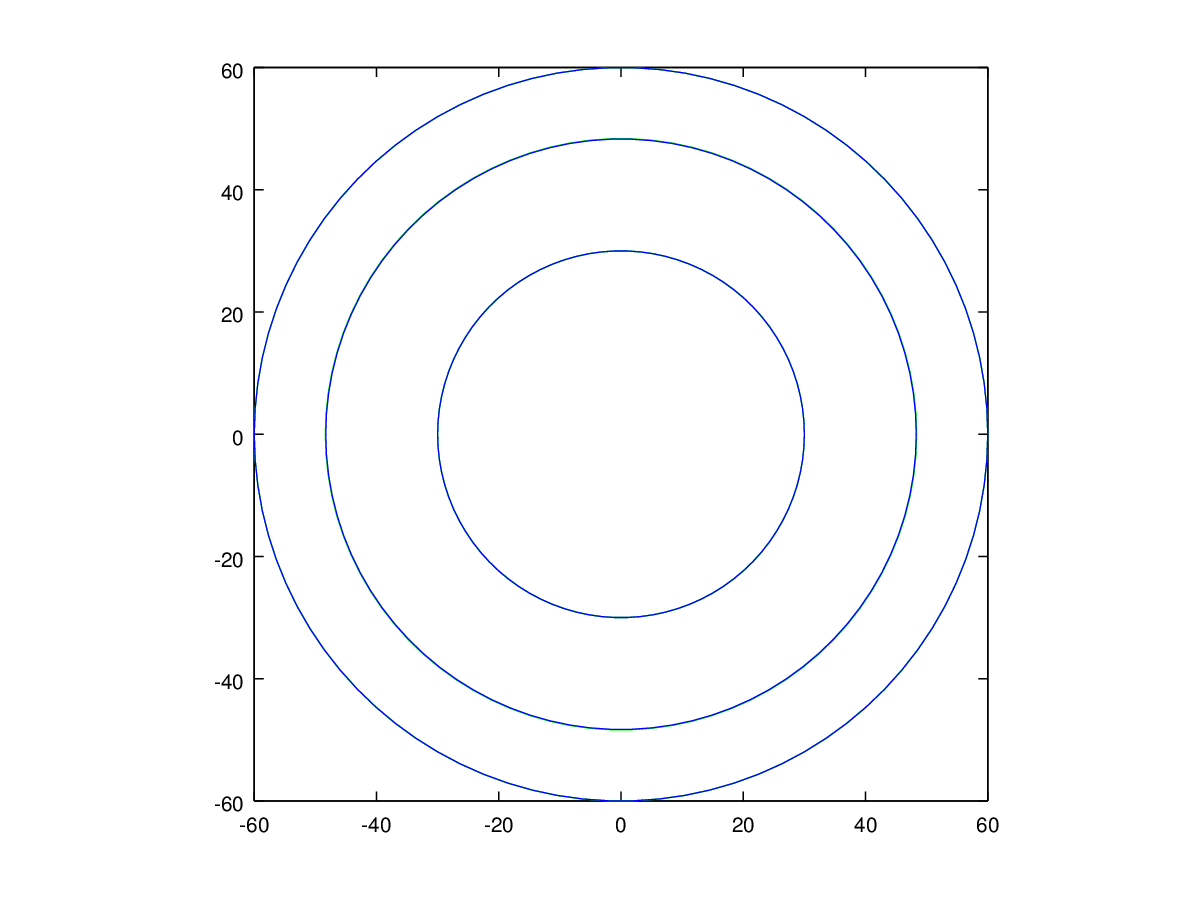
\includegraphics[width=4.5cm]{graficos/1/1b-8-iso.png} &
      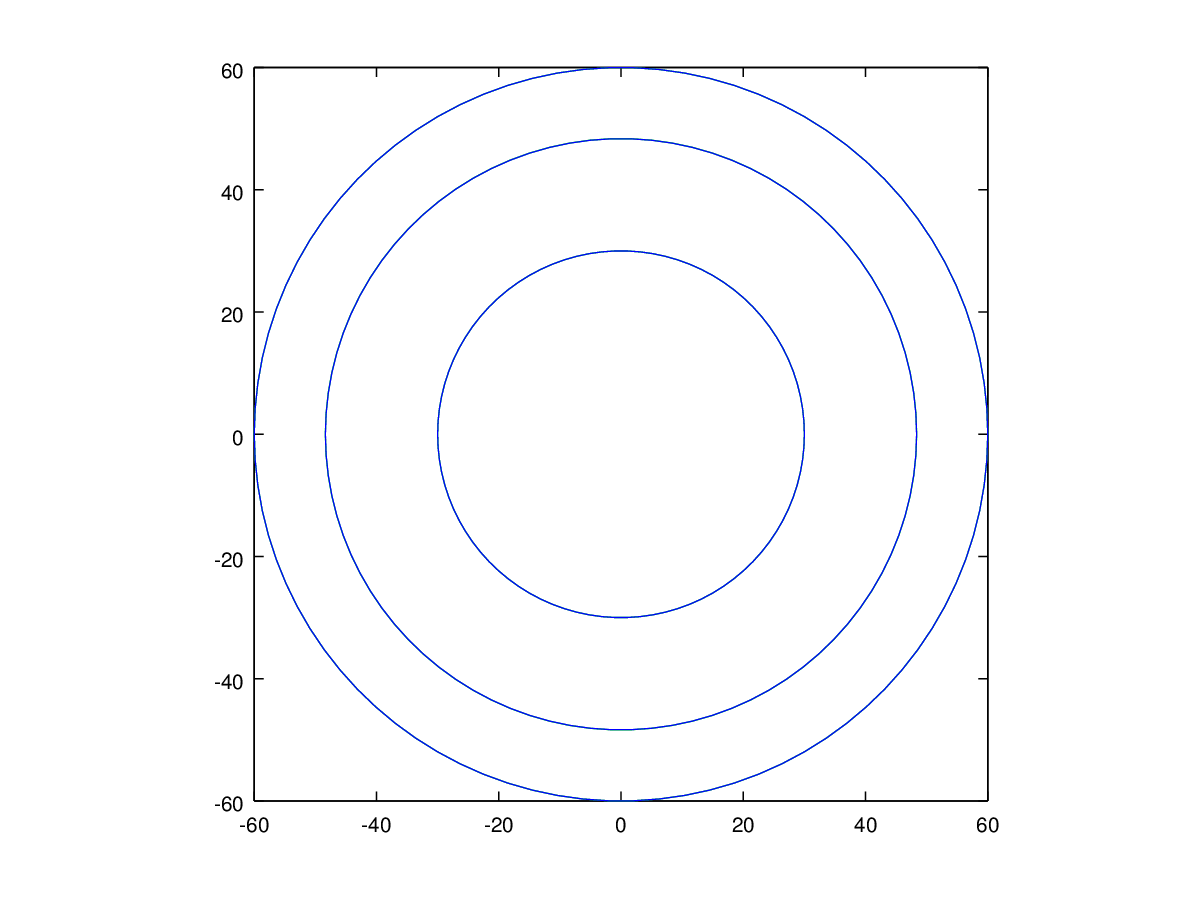
\includegraphics[width=4.5cm]{graficos/1/1b-30-iso.png} \\
      {\small $m+1 = 3$} &
      {\small $m+1 = 8$} &
      {\small $m+1 = 30$} \\
    \end{tabular}}

  \subsubsection*{Experimento 2: Posición de la isoterma según granularidad}

    Para ambos casos se consideraron instancias de prueba con los siguientes parámetros: $r_i = 30$, $r_e = 60$, $T_i = 1500$, $iso = 500$. Se generó una instancia de prueba con una temperatura externa variable entre 50 y 200{\degree}C\footnote{Para la generación de las instancias de prueba se consideró la función $T_e(\theta) = 125 + 75 \sin(2\theta)$} en todos los puntos $(r_e, \theta)$ de la discretización.

    En primer lugar, se calculó la solución del sistema y la posición estimada de la isoterma para una discretización considerablemente granular, con $m + 1 = 70$ y $n = 90$, para utilizar como caso de contraste. Reproducimos los gráficos que representan las temperaturas calculadas para todos los puntos de la discretización y la ubicación estimada de la isoterma.

    {\centering \begin{tabular}{cc}
      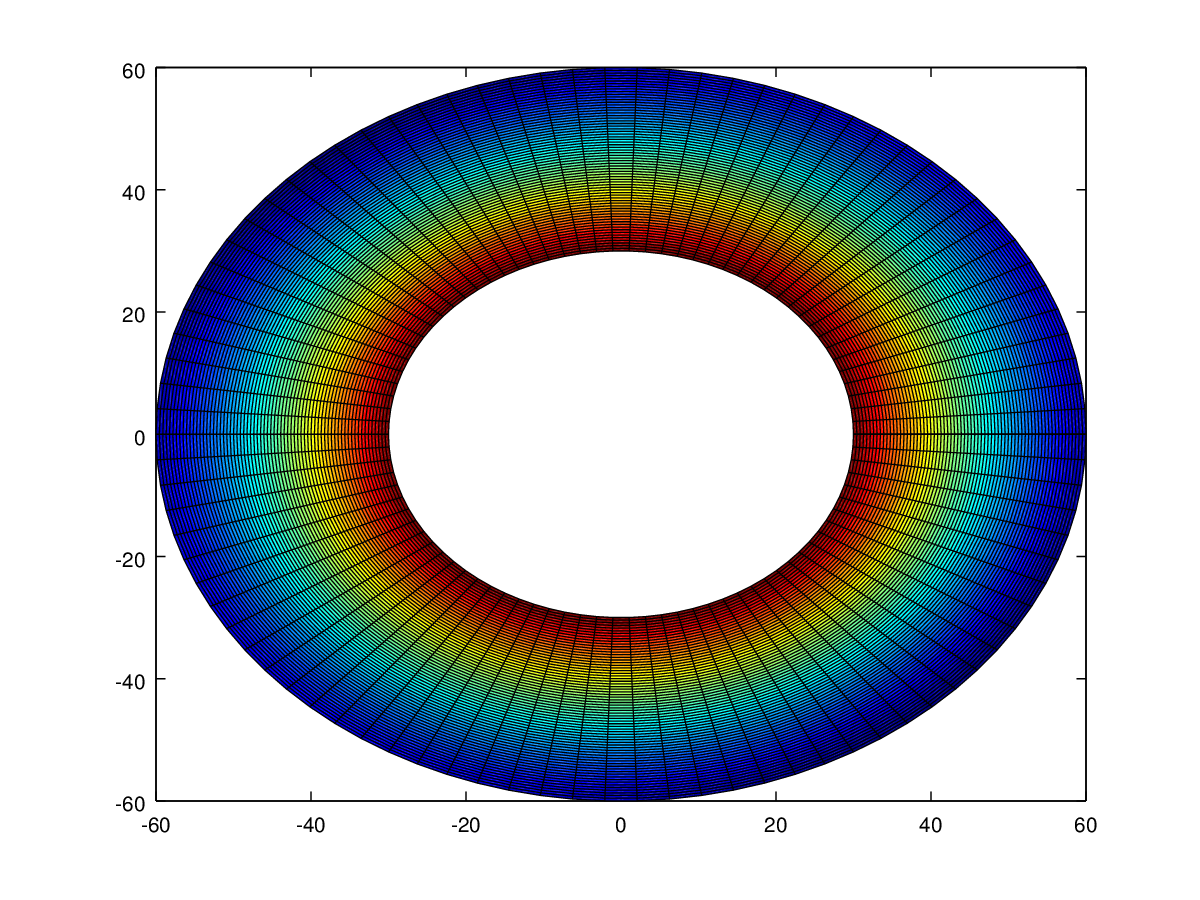
\includegraphics[height=5cm]{graficos/2/2-real.png} & 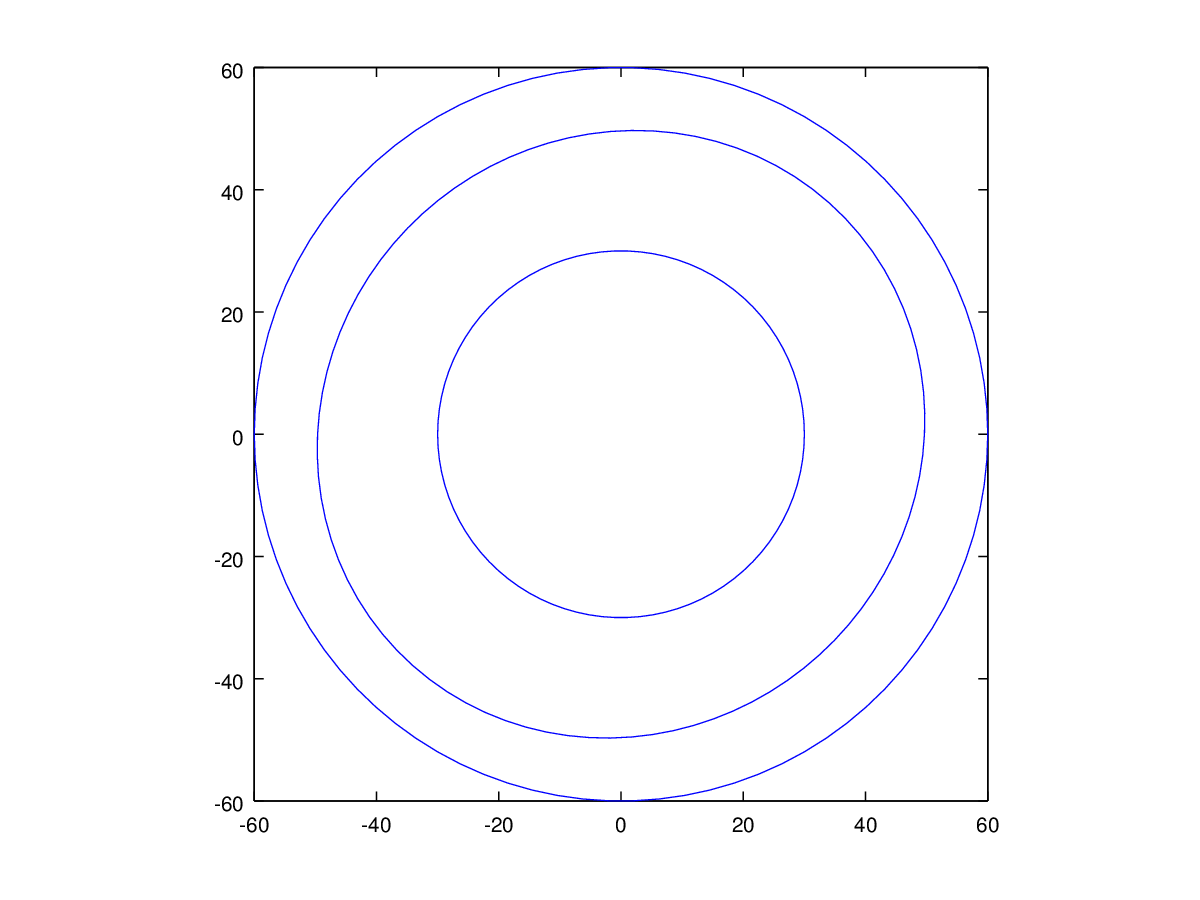
\includegraphics[height=5cm]{graficos/2/2-real-iso.png} \\
      {\small Temperaturas obtenidas} &
      {\small Posición estimada de la isoterma 500{\degree}C} \\
    \end{tabular}}

    \paragraph{Caso A} Se mantuvo constante la cantidad de radios de la discretización $m + 1 = 70$, y se tomaron instancias con diferentes cantidades de ángulos, para $n = 3, 5, 8, 10, 30, 50, 70$. Los gráficos que incluimos representan los resultados obtenidos para $n = 5, 10, 50$, reflejando las temperaturas calculadas y la ubicación estimada de la isoterma (en azul), comparada con la obtenida para el caso de contraste (en verde).

    {\centering \begin{tabular}{ccc}
      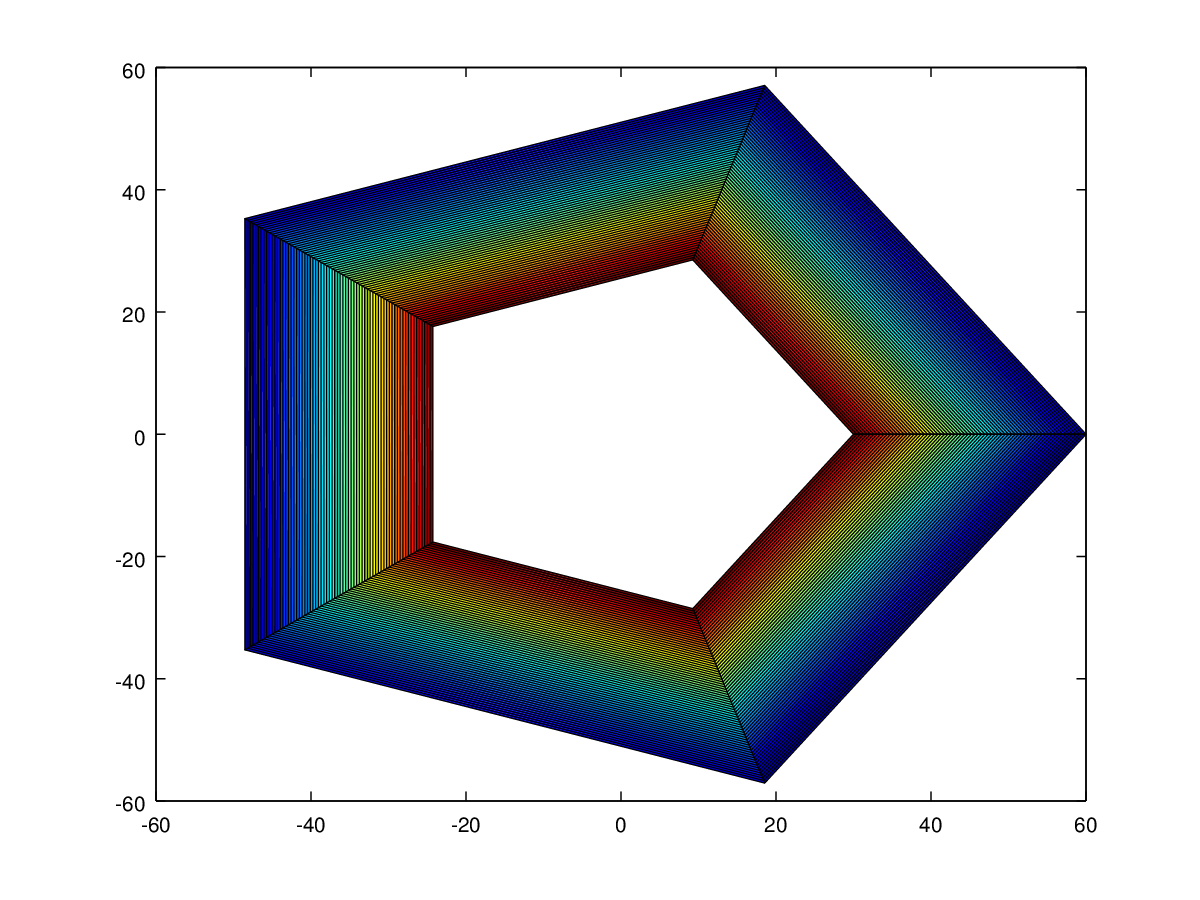
\includegraphics[width=4.5cm]{graficos/2/2a-5.png} &
      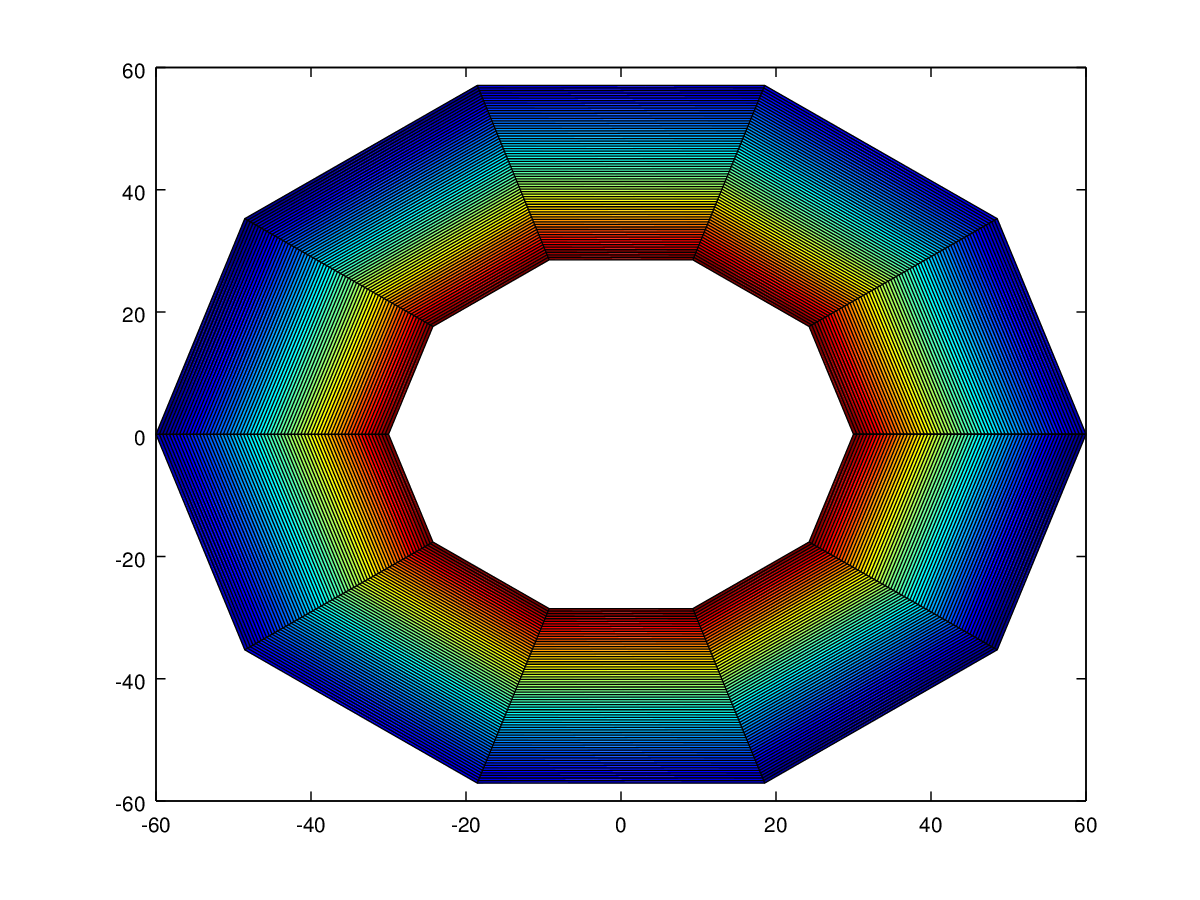
\includegraphics[width=4.5cm]{graficos/2/2a-10.png} &
      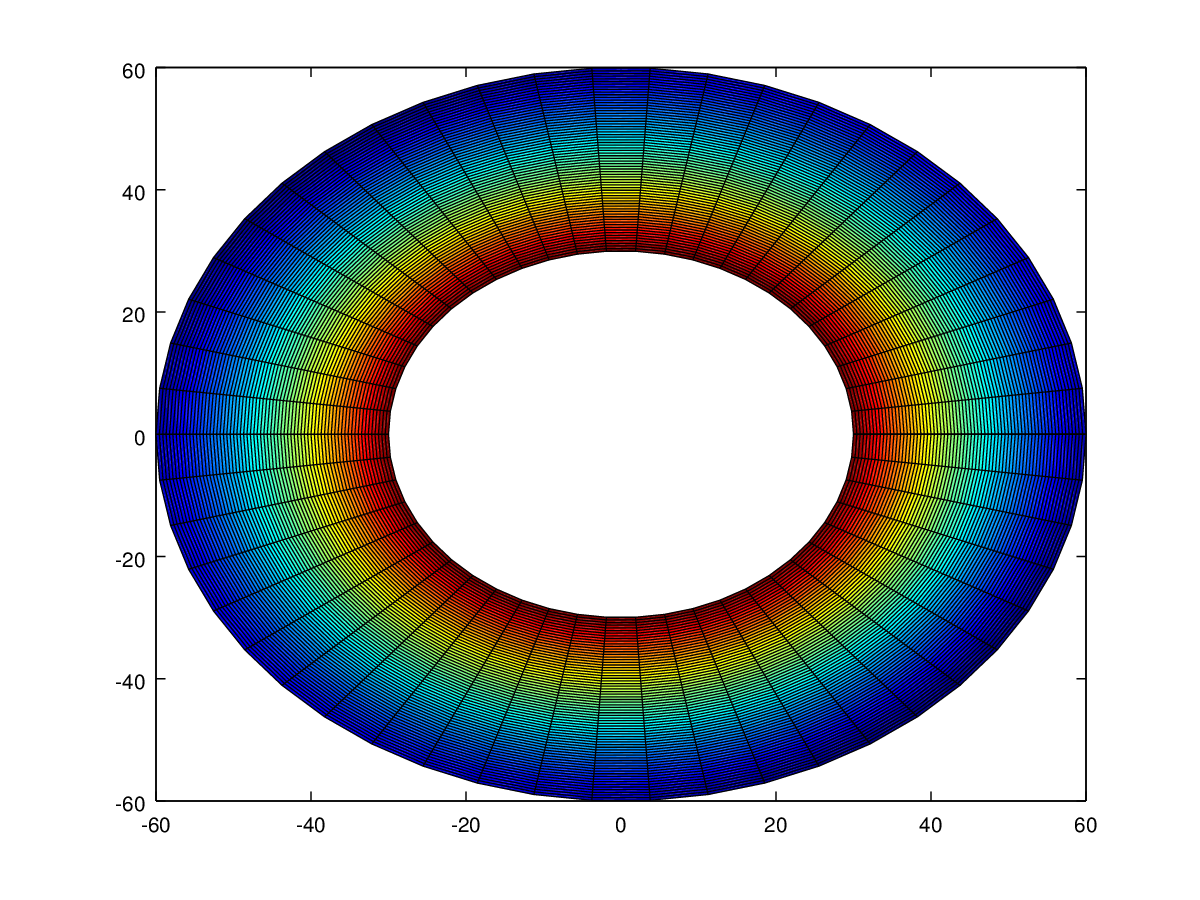
\includegraphics[width=4.5cm]{graficos/2/2a-50.png} \\
      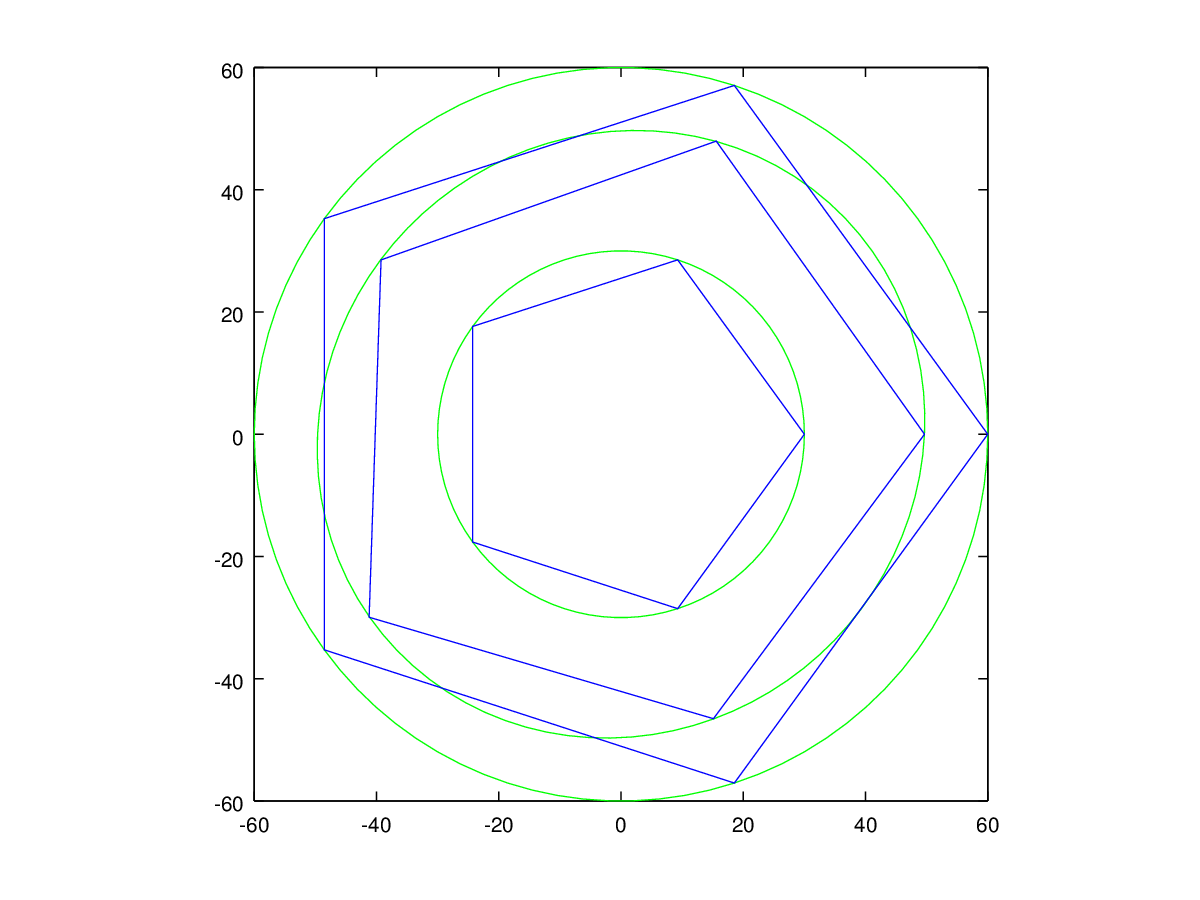
\includegraphics[width=4.5cm]{graficos/2/2a-5-iso.png} &
      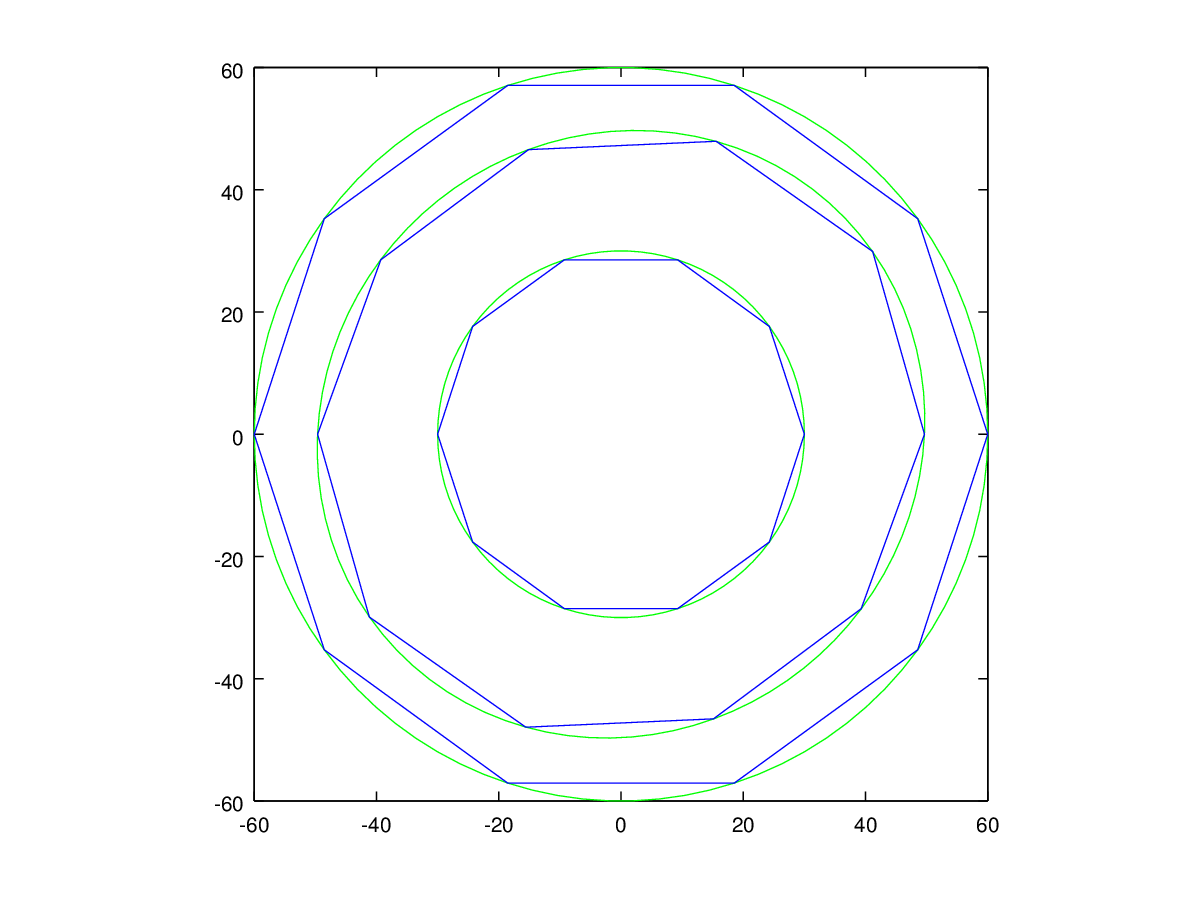
\includegraphics[width=4.5cm]{graficos/2/2a-10-iso.png} &
      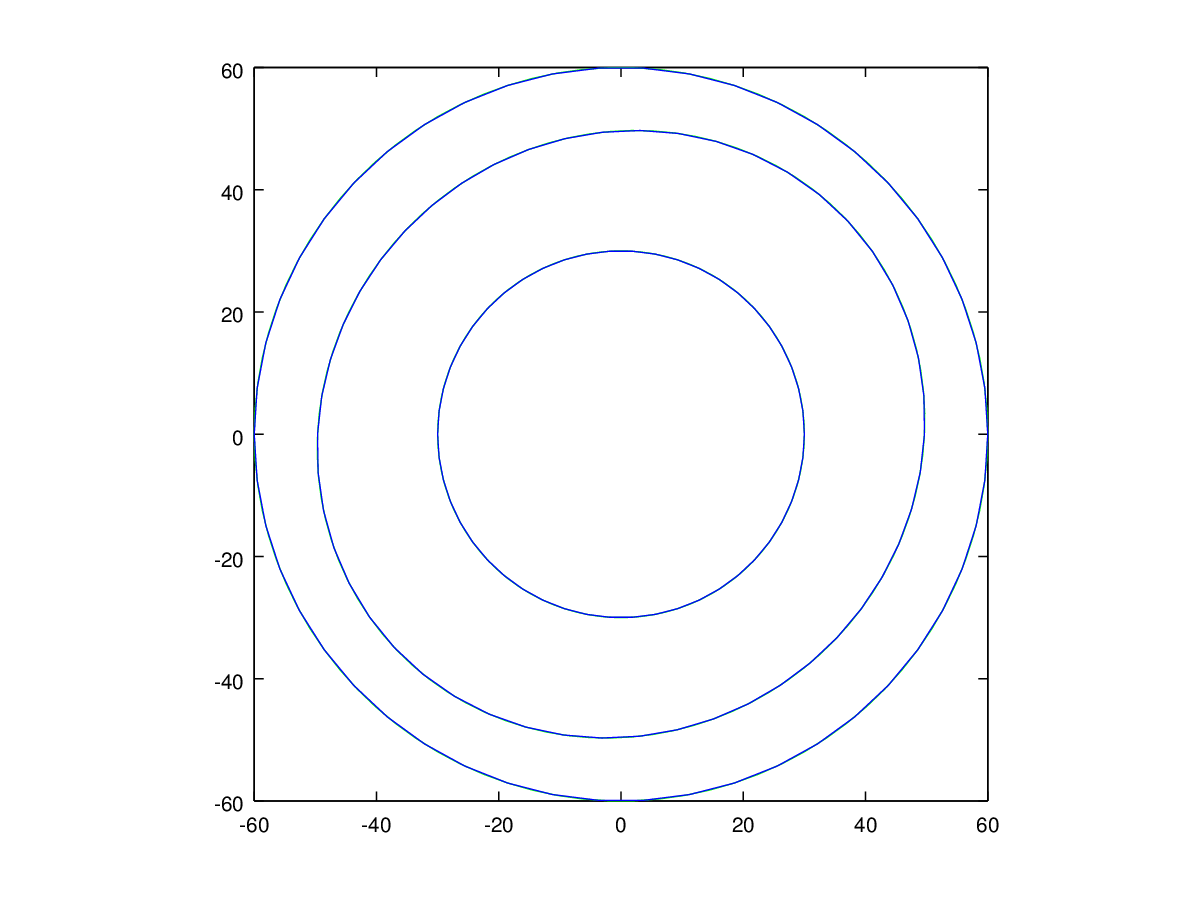
\includegraphics[width=4.5cm]{graficos/2/2a-50-iso.png} \\
      {\small $n = 5$} &
      {\small $n = 10$} &
      {\small $n = 50$} \\
    \end{tabular}}

    \paragraph{Caso B} Se mantuvo constante la cantidad de ángulos de la discretización $n = 90$, y se tomaron instancias con diferentes cantidades de ángulos, para $m + 1 = 3, 5, 8, 10, 30, 50$. Los gráficos que incluimos representan los resultados obtenidos para $m + 1 = 3, 8, 30$, reflejando las temperaturas calculadas y la ubicación estimada de la isoterma (en azul), comparada con la obtenida para el caso de contraste (en verde).

    {\centering \begin{tabular}{ccc}
      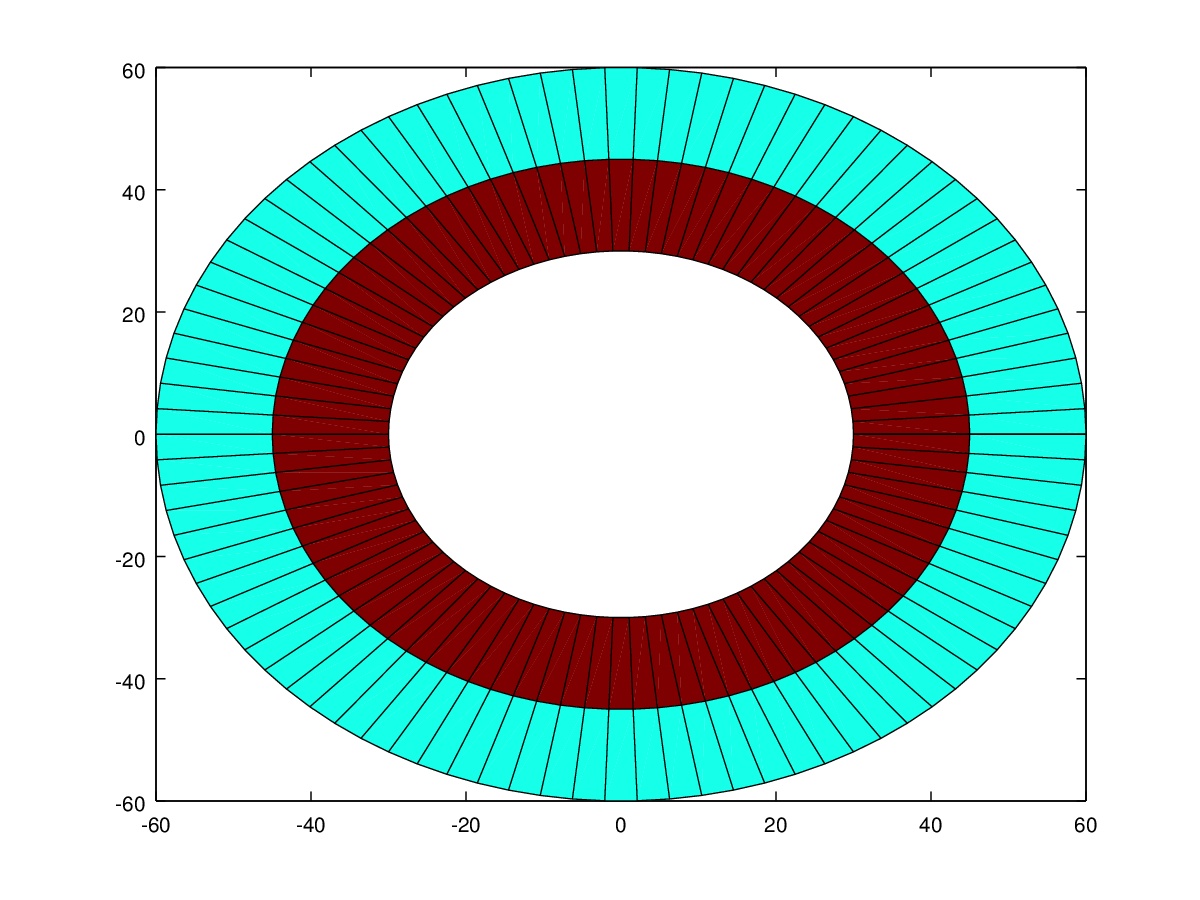
\includegraphics[width=4.5cm]{graficos/1/1b-3.png} &
      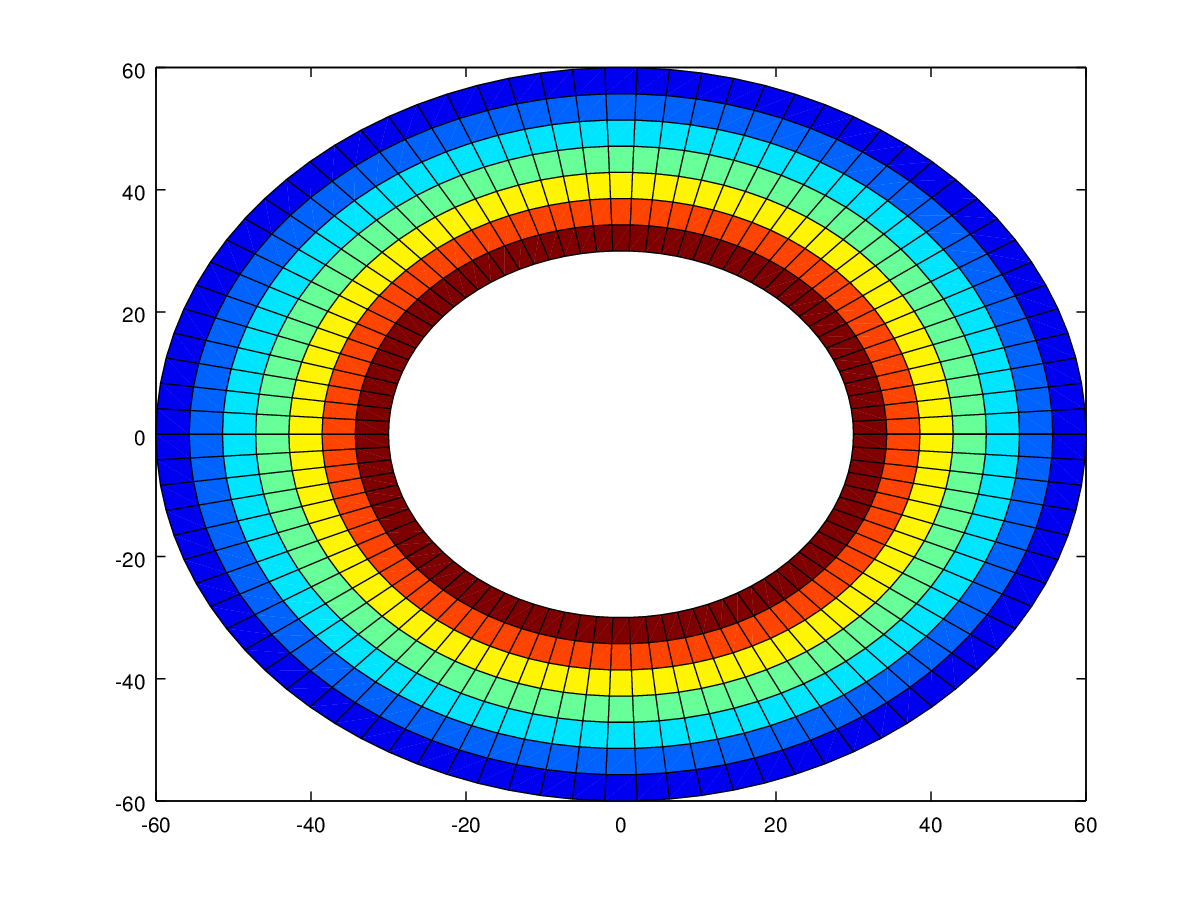
\includegraphics[width=4.5cm]{graficos/1/1b-8.png} &
      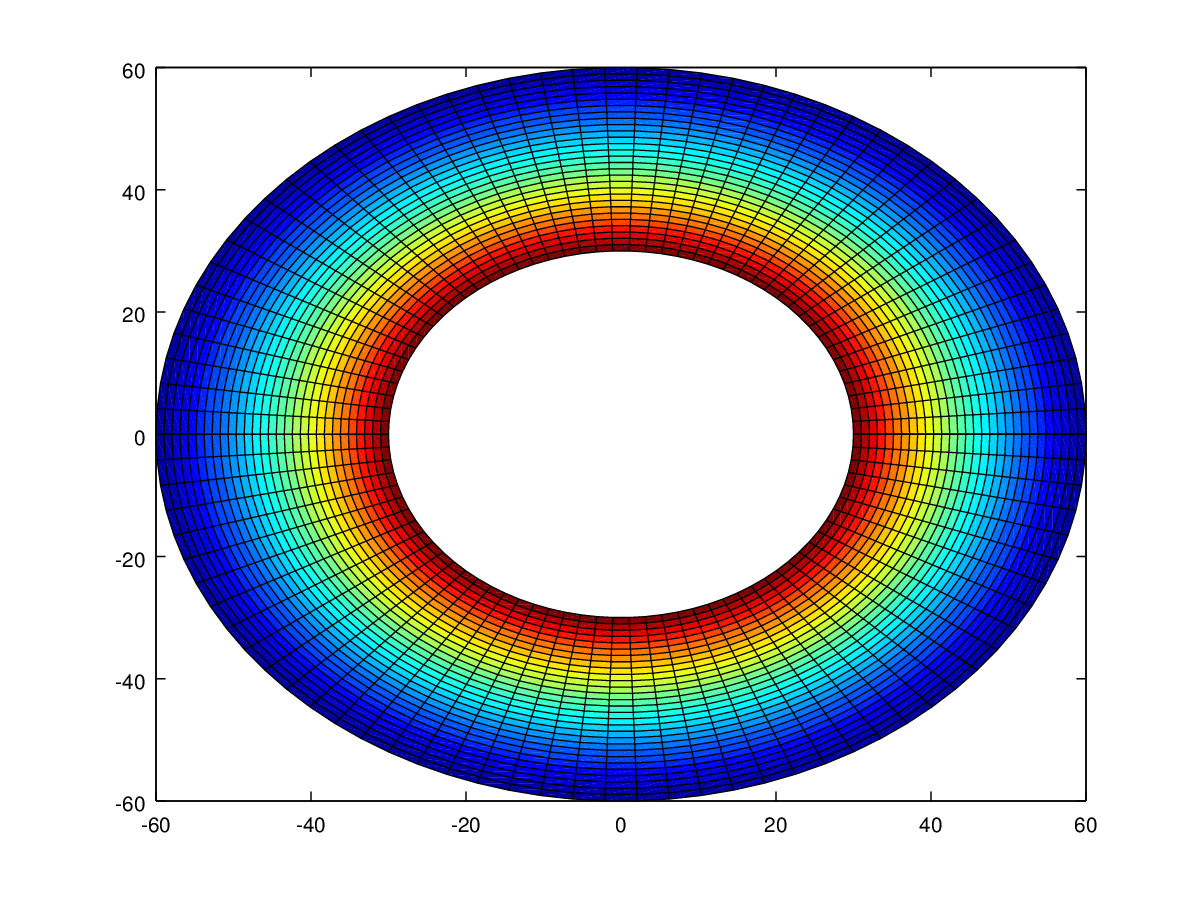
\includegraphics[width=4.5cm]{graficos/1/1b-30.png} \\
      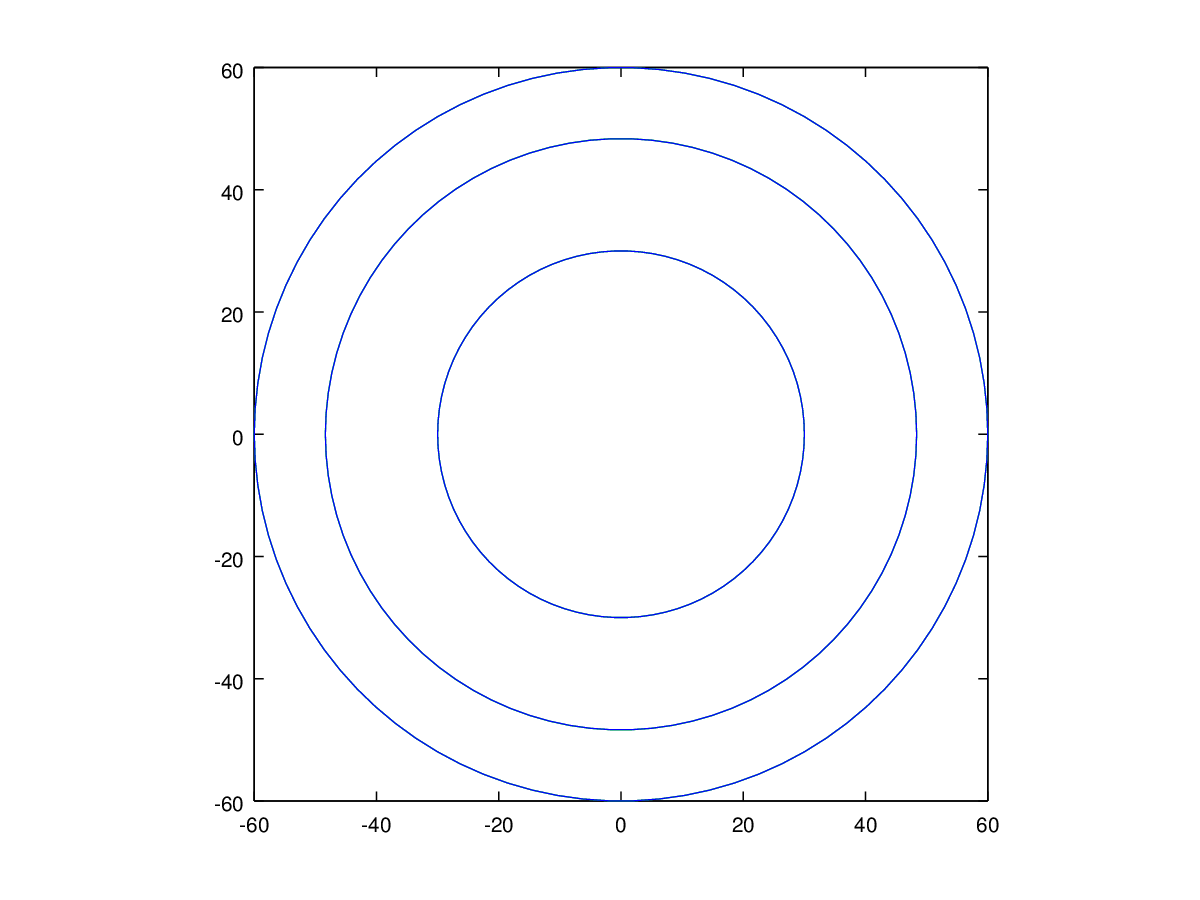
\includegraphics[width=4.5cm]{graficos/1/1b-3-iso.png} &
      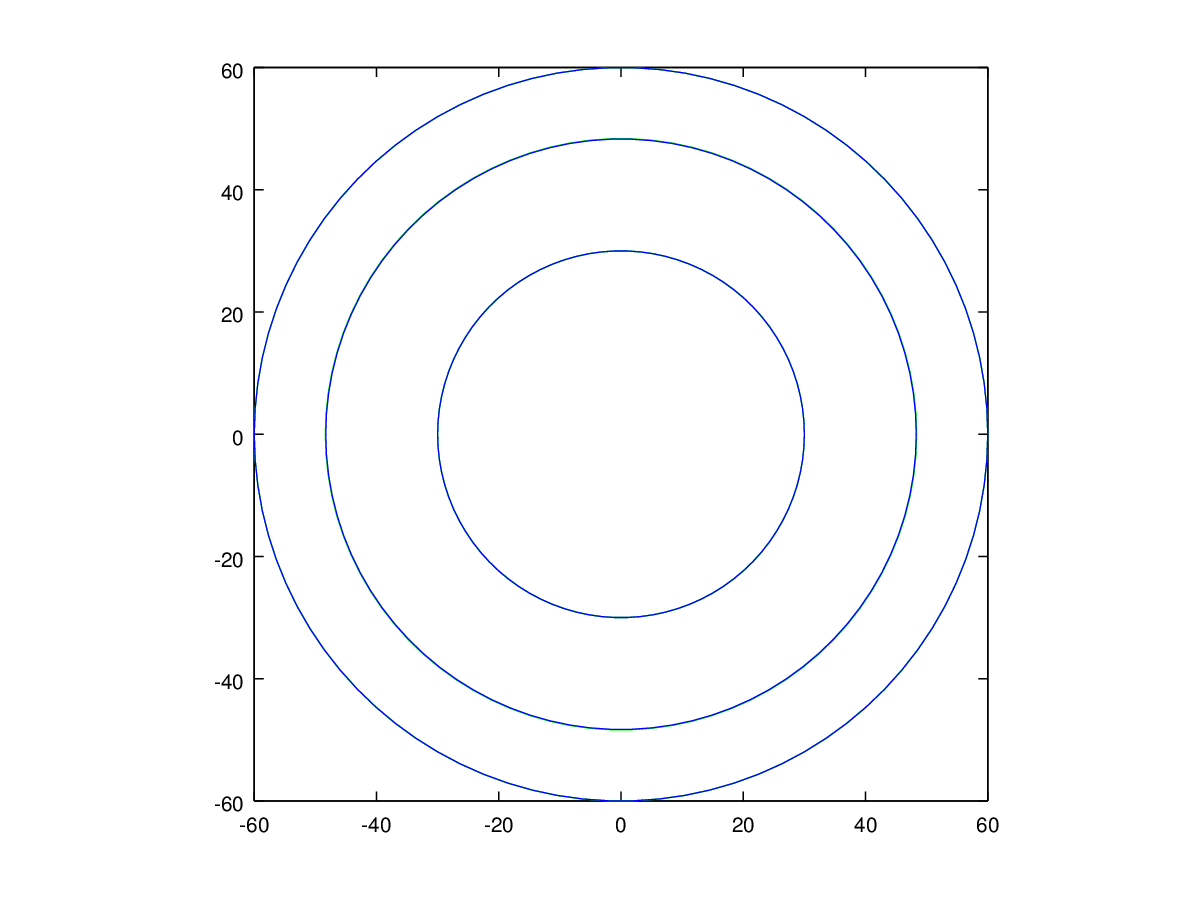
\includegraphics[width=4.5cm]{graficos/1/1b-8-iso.png} &
      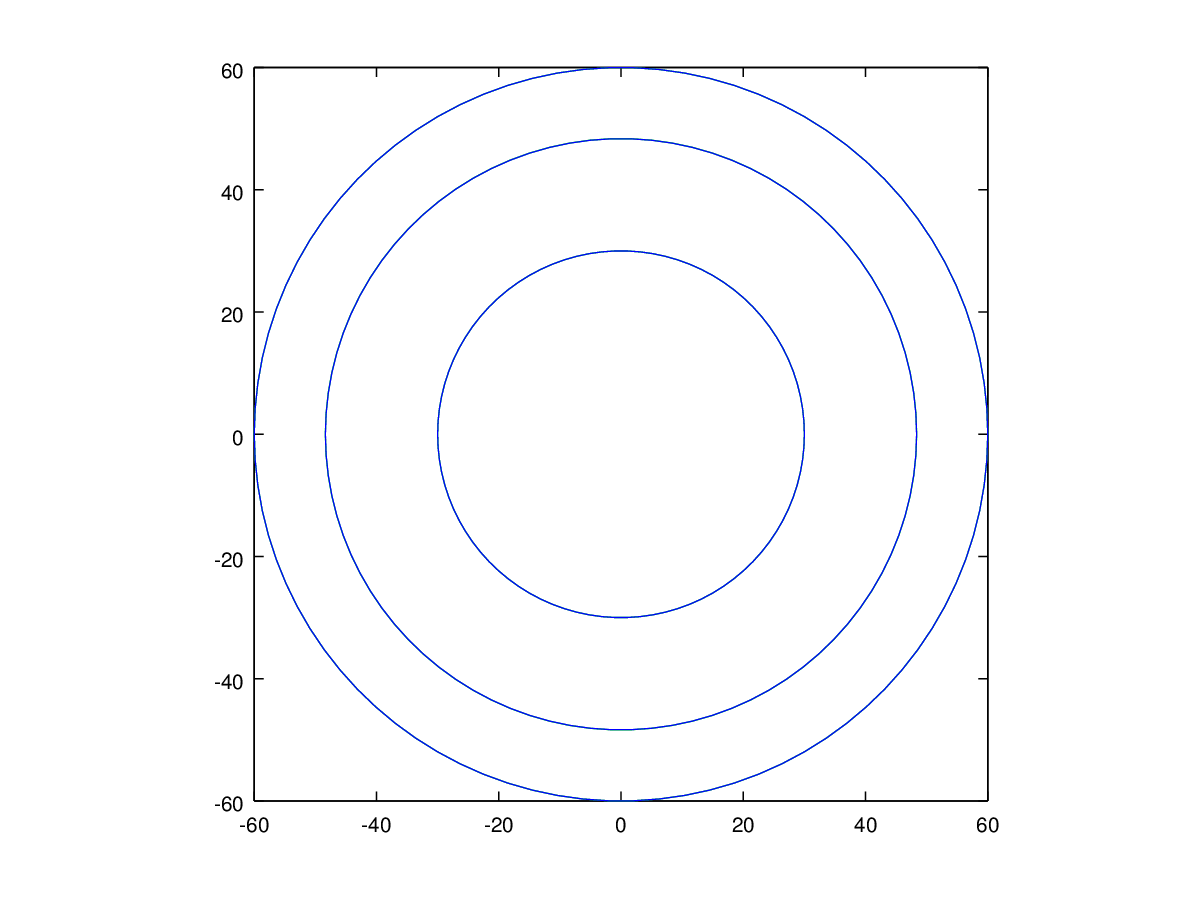
\includegraphics[width=4.5cm]{graficos/1/1b-30-iso.png} \\
      {\small $m+1 = 3$} &
      {\small $m+1 = 8$} &
      {\small $m+1 = 30$} \\
    \end{tabular}}

  \subsubsection*{Experimento 3: Posición de la isoterma según condiciones de borde}

    Se evaluaron dos escenarios de prueba, ambos con los siguientes parámetros: $r_i = 30$, $r_e = 60$, $m+1 = 30$, $n = 30$, $T_i = 1500$, $iso = 500$. Se utilizaron temperaturas externas constantes en todos los puntos $(r_e, \theta)$ de la discretización, con $T_e(\theta) = 50$ en uno de los casos y $T_e(\theta) = 200$ en el otro.

    En el gráfico puede observarse la ubicación estimada de la isoterma para cada uno de los casos, en rojo para $T_e(\theta) = 50$ y en azul para $T_e(\theta) = 200$.

    \begin{center}
      \includegraphics[width=9cm]{graficos/3/3-iso.png} \\
      {\small Posiciones de las isotermas de 500{\degree}C}
    \end{center}

  \subsubsection*{Experimento 4: Índice de peligrosidad según granularidad}

    Se consideró un escenario con los siguientes parámetros: $r_i = 10$, $r_e = 60$, $T_i = 1500$, $iso = 500$. Para la temperatura externa se tomaron valores arbitrarios entre 50 y 200{\degree}C. Luego, se generaron cinco instancias de prueba con los siguientes pares de valores para $m + 1$ y $n$: $(15, 5), (15, 10), (20, 20), (25, 40), (30, 80)$. Se construyó en primer lugar la instancia de prueba con $n = 80$, y las demás se generaron a partir de esta eliminando los valores de $T_e(\theta_k)$ con $k$ par.

    El experimento arrojó los siguientes resultados:

    \begin{center}
      \begin{tabular}{c|c|c}
        $m+1$ & $n$ & Índice de peligrosidad \\ \hline
         15 & 5 & 0.633849 \\
        15 & 10 & 0.633849 \\
        20 & 20 & 0.635172 \\
        25 & 40 & 0.636719 \\
        30 & 80 & 0.637951
      \end{tabular}
    \end{center}

    En el gráfico pueden observarse los valores obtenidos para el índice de peligrosidad de los cinco casos de prueba, en función de la granularidad de la discretización (considerando como medida de la granularidad el valor $(m+1)n$).

    \begin{center}
      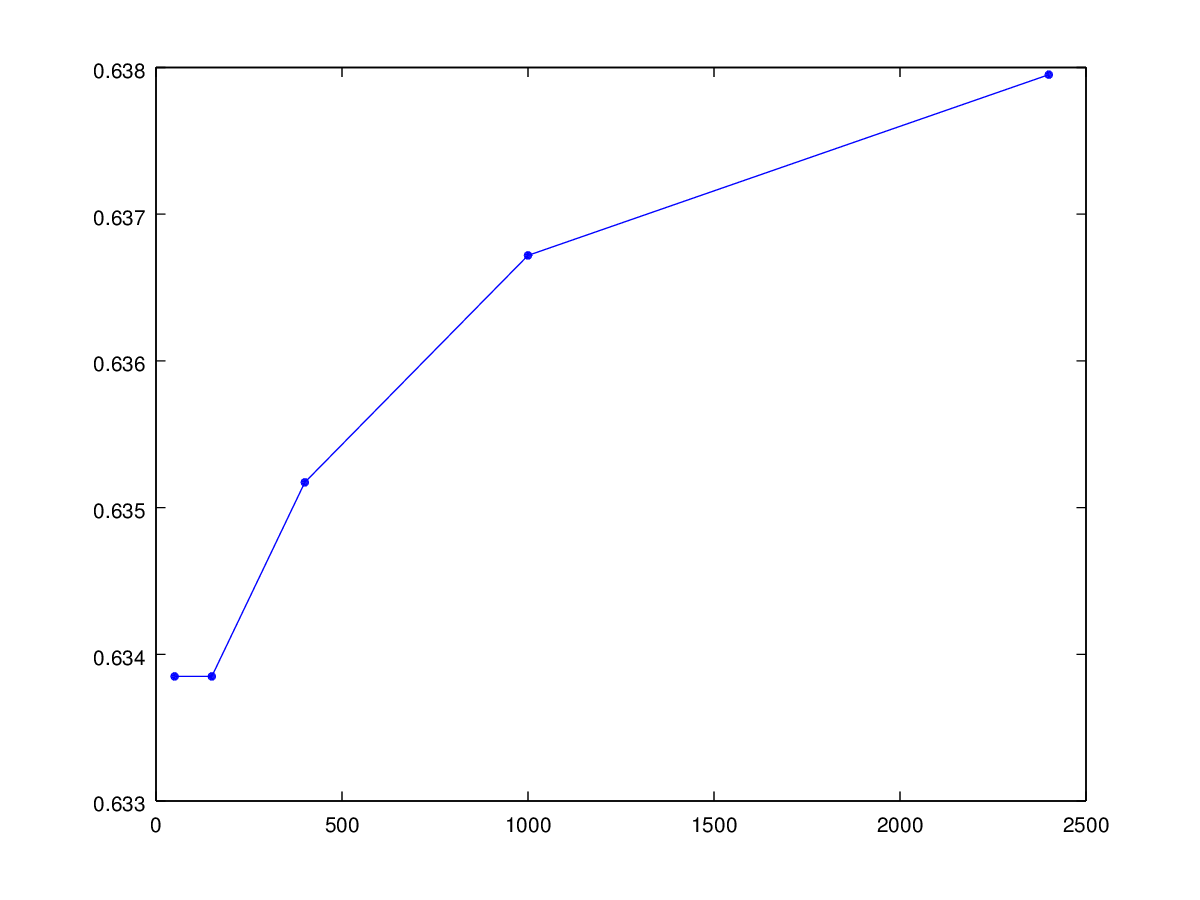
\includegraphics[width=9cm]{graficos/4/4.png} \\
      {\small Índice de peligrosidad en función de la granularidad de la discretización}
    \end{center}

  \subsubsection*{Experimento 5: Índice de peligrosidad según ancho de la pared}

    Para este experimento se mantuvieron constantes los parámetros, $r_e = 90$, $m+1 = 30$, $n = 80$, $T_i = 1500$, $iso = 500$, como así también la temperatura externa $T_e(\theta)$, para la cual se tomaron valores arbitrarios entre 50 y 200{\degree}C. Se generaron instancias con los siguientes valores de $r_i$: $5, 10, 20, 40, 60, 80, 90$. El experimento arrojó los siguientes resultados:

    \begin{center}
      \begin{tabular}{c|c}
        $r_i$ & Índice de peligrosidad \\ \hline
        5 & 0.441240 \\
        10 & 0.557452 \\
        20 & 0.683942 \\
        40 & 0.822686 \\
        60 & 0.909080 \\
        80 & 0.973116 \\
        90 & 1.000000
      \end{tabular}
    \end{center}

    En el gráfico pueden observarse los valores obtenidos para el índice de peligrosidad en función de los diferentes valores de $r_i$.

    \begin{center}
      \includegraphics[width=9cm]{graficos/5/5.png} \\
      {\small Índice de peligrosidad en función del valor de $r_i$}
    \end{center}

  \subsubsection*{Experimento 6: Tiempo de ejecución según número de instancias}

    Se consideró una serie de 6 instancias del problema con los siguientes parámetros: $r_i = 10$, $r_e = 60$, $m+1 = 25$, $n = 40$, $T_i = 1500$, $iso = 500$. Para las temperaturas externas se tomaron valores arbitrarios entre 50 y 200{\degree}C, diferentes en cada una de las instancias.

    Se procesaron sucesivamente 1, 2, 3, 4, 5 y 6 instancias en corridas únicas del programa, utilizando primero el método de Eliminación Gaussiana y luego el de Factorización LU. Los tiempos de ejecución se tomaron en segundos, utilizando la librería \texttt{ctime} de \texttt{C++}. Para las pruebas se omitió realizar la estimación de la posición de la isoterma, limitándose a resolver el sistema por el método elegido. Los valores obtenidos fueron los siguientes:

      \begin{center}
        \begin{tabular}{c|c|c}
          \multirow{2}{*}{$ninst$} & \multicolumn{2}{c}{Tiempo de ejecución(segundos)} \\ 
          & Eliminación Gaussiana & Factorización LU \\ \hline
          1 & 3.099746 & 3.088397 \\
          2 & 6.204906 & 3.089928 \\
          3 & 9.333475 & 3.107586 \\
          4 & 12.392685 & 3.109775 \\
          5 & 15.497981 & 3.119630 \\
          6 & 18.562135 & 3.123978 \\
        \end{tabular}
      \end{center}

    \begin{center}
      \includegraphics[width=9cm]{graficos/6/6.png} \\
      {\small Tiempo de ejecución en función del número de instancias del problema}
    \end{center}

  \subsubsection*{Experimento 7: Tiempo de ejecución según granularidad}

    Para ambos casos, se construyeron escenarios de prueba con los siguientes parámetros: $r_i = 30$, $r_e = 60$, $T_i = 1500$, $iso = 500$. La temperatura externa se consideró constante, con $T_e(\theta) = 50$ para todo $\theta$. En ambos casos las pruebas se realizaron utilizando primero el método de Eliminación Gaussiana y luego el de Factorización LU, y los tiempos de ejecución se tomaron en segundos, utilizando la librería \texttt{ctime} de \texttt{C++}. Para las pruebas se omitió realizar la estimación de la posición de la isoterma, limitándose a resolver el sistema por el método elegido.

    \paragraph{Caso A}
      Se realizaron pruebas variando la cantidad de ángulos de la discretización, con $m + 1 = 30$ y $n = 10, 30, 50, 70, 90$. Los valores obtenidos fueron los siguientes:

      \begin{center}
        \begin{tabular}{c|c|c}
          \multirow{2}{*}{$n$} & \multicolumn{2}{c}{Tiempo de ejecución(segundos)} \\ 
          & Eliminación Gaussiana & Factorización LU \\ \hline
          10 & 0.09335425 & 0.09196125 \\
          30 & 2.25882775 & 2.25695850 \\
          50 & 10.40710775 & 10.40538050 \\
          70 & 28.47581550 & 28.50210100 \\
          90 & 60.43221975 & 60.50333525 \\
        \end{tabular}
      \end{center}

      \begin{center}
        \includegraphics[width=9cm]{graficos/7/7a.png} \\
        {\small Tiempo de ejecución en función de la cantidad de ángulos de la discretización}
      \end{center}

    \paragraph{Caso B}
      Se realizaron pruebas variando la cantidad de radios de la discretización, con $n = 60$ y $m+1 = 10, 30, 50, 70$. Los valores obtenidos fueron los siguientes:

      \begin{center}
        \begin{tabular}{c|c|c}
          \multirow{2}{*}{$m + 1$} & \multicolumn{2}{c}{Tiempo de ejecución(segundos)} \\ 
          & Eliminación Gaussiana & Factorización LU \\ \hline
          10 & 0.67524000 & 0.67400350 \\
          30 & 17.94450675 & 17.98105550 \\
          50 & 82.86414400 & 83.05790825 \\
          70 & 227.07038100 & 227.68770850 \\
        \end{tabular}
      \end{center}

      \begin{center}
        \includegraphics[width=9cm]{graficos/7/7b.png} \\
        {\small Tiempo de ejecución en función de la cantidad de radios de la discretización}
      \end{center}
